%\documentclass[compress]{beamer}
\documentclass{beamer}

% Try the class options [notes], [notes=only], [trans], [handout],
% [red], [compress], [draft], [class=article] and see what happens!

% For a green structure color use:
\colorlet{structure}{green!50!black}

\mode<article> % only for the article version
{
  \usepackage{beamerbasearticle}
  \usepackage{fullpage}
  \usepackage{hyperref}
}



\beamertemplateshadingbackground{red!10}{blue!10}

\setbeamertemplate{footline}[page number]
\usepackage{beamerthemeshadow}

\usepackage{pgf,pgfarrows,pgfnodes,pgfautomata,pgfheaps,pgfshade}
\usepackage{graphicx}
\usepackage{amsmath,amssymb}
\usepackage[latin1]{inputenc}
\usepackage{colortbl}
\usepackage[english]{babel}


%\usepackage{times}

% Use some nice templates
\beamertemplatetransparentcovereddynamic

% own commands

\newcommand{\be}{\begin{equation}}
\newcommand{\ee}{\end{equation}}
\newcommand{\bra}[1]{\left\langle #1 \right|}
\newcommand{\ket}[1]{\left| #1 \right\rangle}
\newcommand{\braket}[2]{\left\langle #1 \right| #2 \right\rangle}
\newcommand{\OP}[1]{{\bf\widehat{#1}}}
\newcommand{\matr}[1]{{\bf \cal{#1}}}
\def\d{\text{d}}
\def\sech{\text{sech}}
\def\Cdot{\!\cdot\!} 
\def\e{\text{e}}
\def\L_2{\L_{2}}
\def\fm{\:\:\mathrm{fm}^{-1}}

%\newcommand{\braket}[1]{\langle#1\rangle}
%\newcommand{\Span}{\operatorname{sp}}
%\newcommand{\tr}{\operatorname{trace}}
%\newcommand{\diag}{\operatorname{diag}}

\newcommand{\pdiff}[2]{\frac{\partial#1}{\partial#2}}
\newcommand{\wedgeprod}[2]{\overset{#2}{\underset{#1}{\wedge}}}
\newcommand{\directsum}[2]{\overset{#2}{\underset{#1}{\bigoplus}}}
\newcommand{\Span}{\operatorname{span}}
\newcommand{\Hilb}{{\mathcal{H}}}
\newcommand{\Proj}{{\mathcal{P}}}
\newcommand{\Model}{{\mathcal{M}}}
\newcommand{\CalS}{{\mathcal{S}}}
\newcommand{\PhiFD}{\Phi^\mathrm{FD}}
\newcommand{\Ind}{{\mathcal{I}}}
\newcommand{\rmd}{\mathrm{d}}
\newcommand{\sgn}{\operatorname{sgn}}
\newcommand{\eofproof}{\hspace{1em}$\diamondsuit$}

\usetheme{Copenhagen}
%\useinnertheme{rectangle}
\title{Coulomb interaction driven entanglement of electrons on helium, theory and experiment}
\author{Morten Hjorth-Jensen\inst{1,2}}
\institute{Department of Physics and Astronomy and Facility for Rare Isotope Beams (FRIB), Michigan State University, USA\inst{1}
\and
Department of Physics, University of Oslo, Norway\inst{2}}
\date{January 20-21, 2025, Nordic Quantum Meeting}

\begin{document}

\frame{\titlepage}

%\section<presentation>*{Outline}
%
%\frame
%{
%  \frametitle{Outline}
%  \tableofcontents[part=1,pausesections]
%  \tableofcontents[part=1]
%}

%\AtBeginSubsection[]
%{
%  \frame<handout:0>
%  {
%    \frametitle{Outline}
%    \tableofcontents[current,currentsubsection]
%  }
%}

\part<presentation>{Main Talk}


%\frame{\titlepage}

%\frame{\tableofcontents}

%\part<presentation>{Main Talk}


\section{Introduction and motivation}

\begin{frame}[plain,fragile]
\frametitle{Overview and Motivation}

\textbf{How to use many-body theory to design quantum circuits (Quantum engineering)}
\begin{enumerate}
\item Many-body methods like F(ull)C(onfiguration)I(nteraction) theory  with
\begin{itemize}

  \item Time dependence

  \item Optimization of experimental parameters 

  \item Feedback from experiment

\end{itemize}
\item Finding optimal parameters for tuning of entanglement
\end{enumerate}

\noindent
\end{frame}

\begin{frame}[plain,fragile]
\frametitle{Collaborators and people to thank}

\begin{block}{MSU }
Niyaz Beysengulov and Johannes Pollanen (experiment, Physics); Zachary Stewart, Jared Weidman, and Angela Wilson (quantum chemistry), Dean Lee, Patrick Cook, Danny Jammooa, Nicholas Cariello, and Aymeric McRau (theory)
\end{block}
\begin{block}{University of Oslo }
Jonas B. Flaten, Oskar M. Leinonen, Christopher Linder\"alv, H\aa kon Kvernmoen, \O yvind Sigmundson Sch\o yen, Stian Dysthe Bilek, and H\aa kon Emil Kristiansen (Physics and quantum chemistry).
\end{block}
\end{frame}

\begin{frame}[plain,fragile]
\frametitle{What is this talk about?}
\begin{block}{}
Here we describe a method for generating motional entanglement between
electrons trapped above the surface of superfluid helium. In this
proposed scheme these electronic charge qubits are laterally confined
via electrostatic gates to create an anharmonic trapping
potential. When the system is cooled to sufficiently low temperature
these in-plane charge qubit states are quantized and circuit quantum
electrodynamic methods can be used to control and readout single qubit
operations. Perspectives for quantum simulations with quantum dots
systems will be discussed.
\end{block}
\end{frame}

\begin{frame}[plain,fragile]
\frametitle{Literature and more reading}

\begin{block}{}
\begin{enumerate}
\item EEROQ corporation at \href{{https://eeroq.com/}}{\nolinkurl{https://eeroq.com/}}

\item Pollanen and many other, Accelerating Progress Towards Practical Quantum Advantage: The Quantum Technology Demonstration Project Roadmap \href{{https://arxiv.org/pdf/2210.14757.pdf}}{\nolinkurl{https://arxiv.org/pdf/2210.14757.pdf}}

\item Original inspiration a series of articles of Loss and DiVincenzo from the nineties, Quantum Computation with Quantum Dots \href{{https://journals.aps.org/pra/pdf/10.1103/PhysRevA.57.120}}{\nolinkurl{https://journals.aps.org/pra/pdf/10.1103/PhysRevA.57.120}}

\item N.R.~Beysengulov, J.~Pollanen, \O .S.~Sch\o yen, S.D.~Bilek, J.B.~Flaten, O.M.~Leinonen, H.E.~Kristiansen, Z.J.~Stewart, J.D.~Weidman, A.K.~Wilson, M.~Hjorth-Jensen, Coulomb interaction-driven entanglement of electrons on helium, PRX Quantum 5, 030324 (2024) and \href{{https://journals.aps.org/prxquantum/abstract/10.1103/PRXQuantum.5.030324}}{\nolinkurl{https://journals.aps.org/prxquantum/abstract/10.1103/PRXQuantum.5.030324}}
\end{enumerate}

\noindent
\end{block}
\end{frame}

\begin{frame}[plain,fragile]
\frametitle{Di Vincenzo criteria}

\begin{alertblock}{Quantum computing requirements }
\begin{enumerate}
\item A scalable physical system with well-characterized qubit

\item The ability to initialize the state of the qubits to a simple fiducial state

\item Long relevant Quantum coherence times longer than the gate operation time

\item A \textbf{universal} set of quantum gates

\item A qubit-specific measurement capability
\end{enumerate}

\noindent
\end{alertblock}
\end{frame}

\begin{frame}[plain,fragile]
\frametitle{Candidate systems}

\begin{block}{Examples of systems}
\begin{enumerate}
\item Superconducting Josephon junctions

\item Single photons

\item \href{{https://journals.aps.org/rmp/pdf/10.1103/RevModPhys.93.025001}}{Trapped ions and atoms}

\item Nuclear Magnetic Resonance

\item Quantum dots and Point Defects in semiconductors

\item ...more
\end{enumerate}
\end{block}
\end{frame}

\begin{frame}[plain,fragile]
\frametitle{Electrons on superfluid helium (Idealized quantum dot system)}
\begin{block}{}
Electrons on \textbf{superfluid helium represent} (see \href{{https://www.youtube.com/watch?v=EuDuM-fe-lA&ab_channel=JoshuahHeath}}{\nolinkurl{https://www.youtube.com/watch?v=EuDuM-fe-lA&ab_channel=JoshuahHeath}}) a promising platform for investigating
strongly-coupled qubits.
\end{block}
\begin{block}{}
A systematic investigation of the
controlled generation of entanglement between two trapped electrons
under the influence of coherent microwave driving pulses, taking into
account the effects of the Coulomb interaction between electrons, may be of great interest for quantum information processing using
trapped electrons.
\end{block}
\end{frame}

\begin{frame}[plain,fragile]
\frametitle{Additional references}
\begin{block}{Experiments and theory}
\begin{enumerate}
\item See \href{{https://www.nature.com/articles/s41586-022-04539-x}}{Single electrons on solid neon as a solid-state qubit platform, David Schuster et al, Nature \textbf{605}, 4650 (2022)}

\item See Mark Dykman et al, Spin dynamics in quantum dots on liquid helium, PRB \textbf{107}. 035437 (2023) at \href{{https://link.aps.org/doi/10.1103/PhysRevB.107.035437}}{\nolinkurl{https://link.aps.org/doi/10.1103/PhysRevB.107.035437}}.
\end{enumerate}
\end{block}
\end{frame}

\begin{frame}[plain,fragile]
\frametitle{Important properties}

\begin{block}{Electron on helium}
\begin{enumerate}
\item Long coherence times

\item Highly connect qubits

\item Many qubits in a small area

\item CMOS compatible

\item Fast gates
\end{enumerate}
\end{block}
\end{frame}



\frame
    {
      \frametitle{Single electrons can make great qubits}
	
      \begin{footnotesize}
     \begin{columns}
       \column{5.0cm}

       At the heart is the trapping and control
       of individual electrons floating above pools of superfluid
       helium. These electrons form the qubits of our quantum
       computer, and the purity of the superfluid helium protects the
       intrinsic quantum properties of each electron. The  ultimate
       goal is to build a large-scale quantum computer based on
       quantum magnetic (spin) state of these trapped electrons.
\column{5cm}
      \begin{center}
	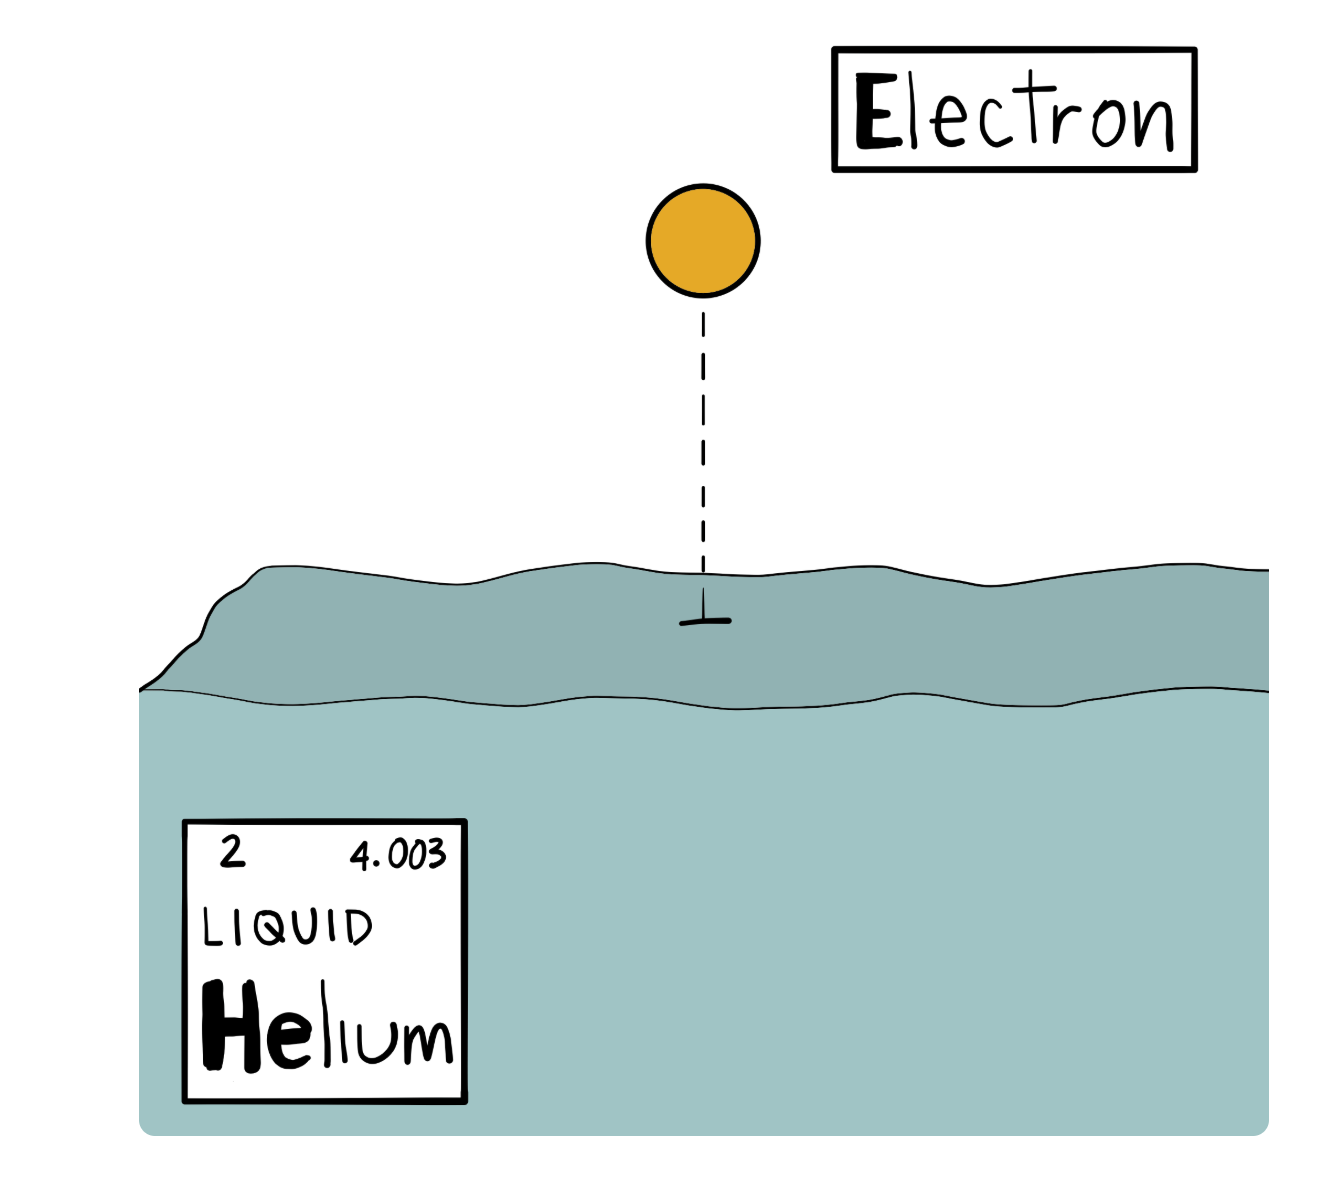
\includegraphics[width=1.2\textwidth]{qcfigures/nordicquantumfig1.png}
      \end{center}
\end{columns}
      \end{footnotesize}
    }


\frame
    {
      \frametitle{Trapping electrons in microchannels}
	
      \begin{footnotesize}
     \begin{columns}
       \column{5.0cm}

       At the heart is the trapping and control
       of individual electrons floating above pools of superfluid
       helium. These electrons form the qubits of our quantum
       computer, and the purity of the superfluid helium protects the
       intrinsic quantum properties of each electron. The  ultimate
       goal is to build a large-scale quantum computer based on
       quantum magnetic (spin) state of these trapped electrons.


\column{5cm}
      \begin{center}
	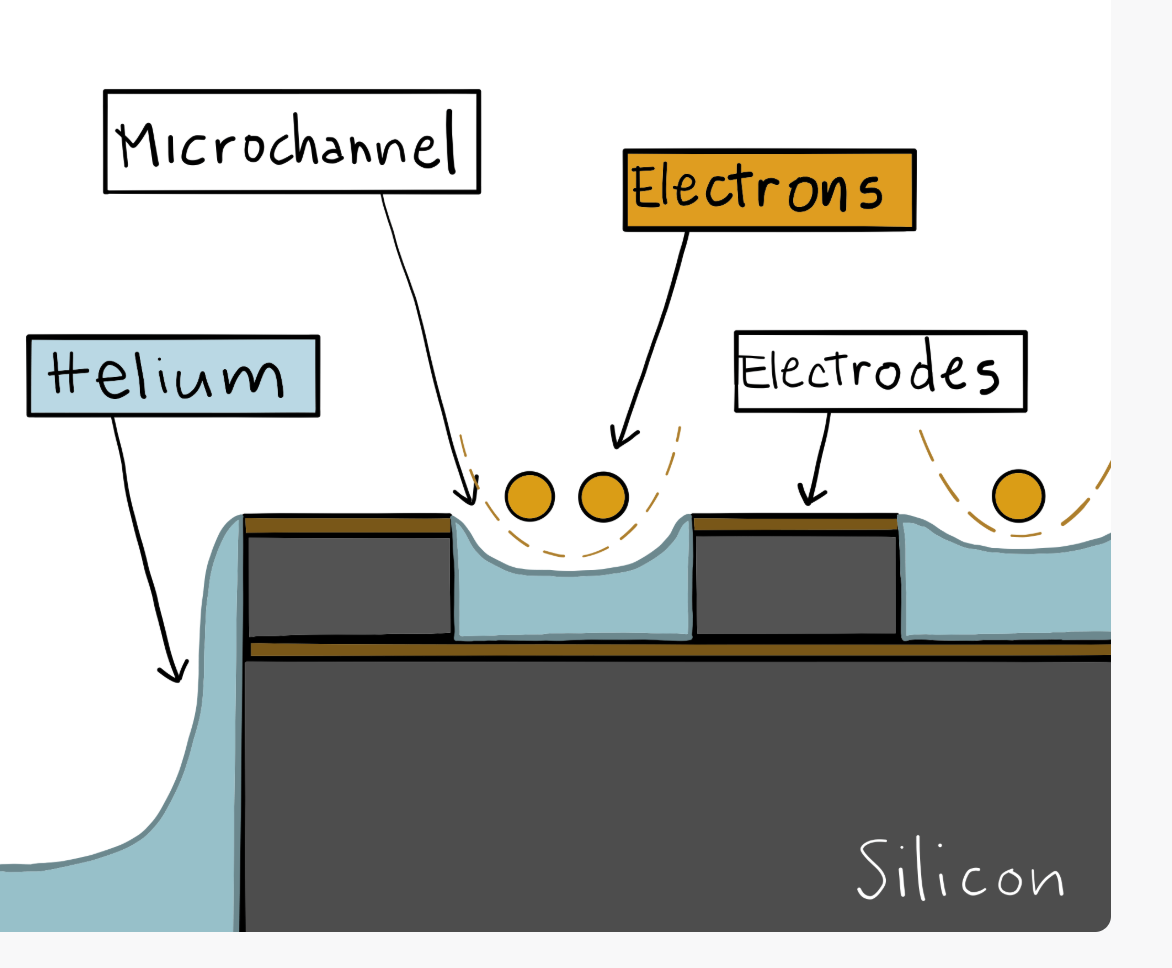
\includegraphics[width=1.2\textwidth]{qcfigures/nordicquantumfig2.png}
      \end{center}
\end{columns}
      \end{footnotesize}
    }

\frame
    {
      \frametitle{Control and readout}
	
      \begin{footnotesize}
     \begin{columns}
       \column{5.0cm}

       At the heart is the trapping and control
       of individual electrons floating above pools of superfluid
       helium. These electrons form the qubits of our quantum
       computer, and the purity of the superfluid helium protects the
       intrinsic quantum properties of each electron. The  ultimate
       goal is to build a large-scale quantum computer based on
       quantum magnetic (spin) state of these trapped electrons.


\column{5cm}
      \begin{center}
	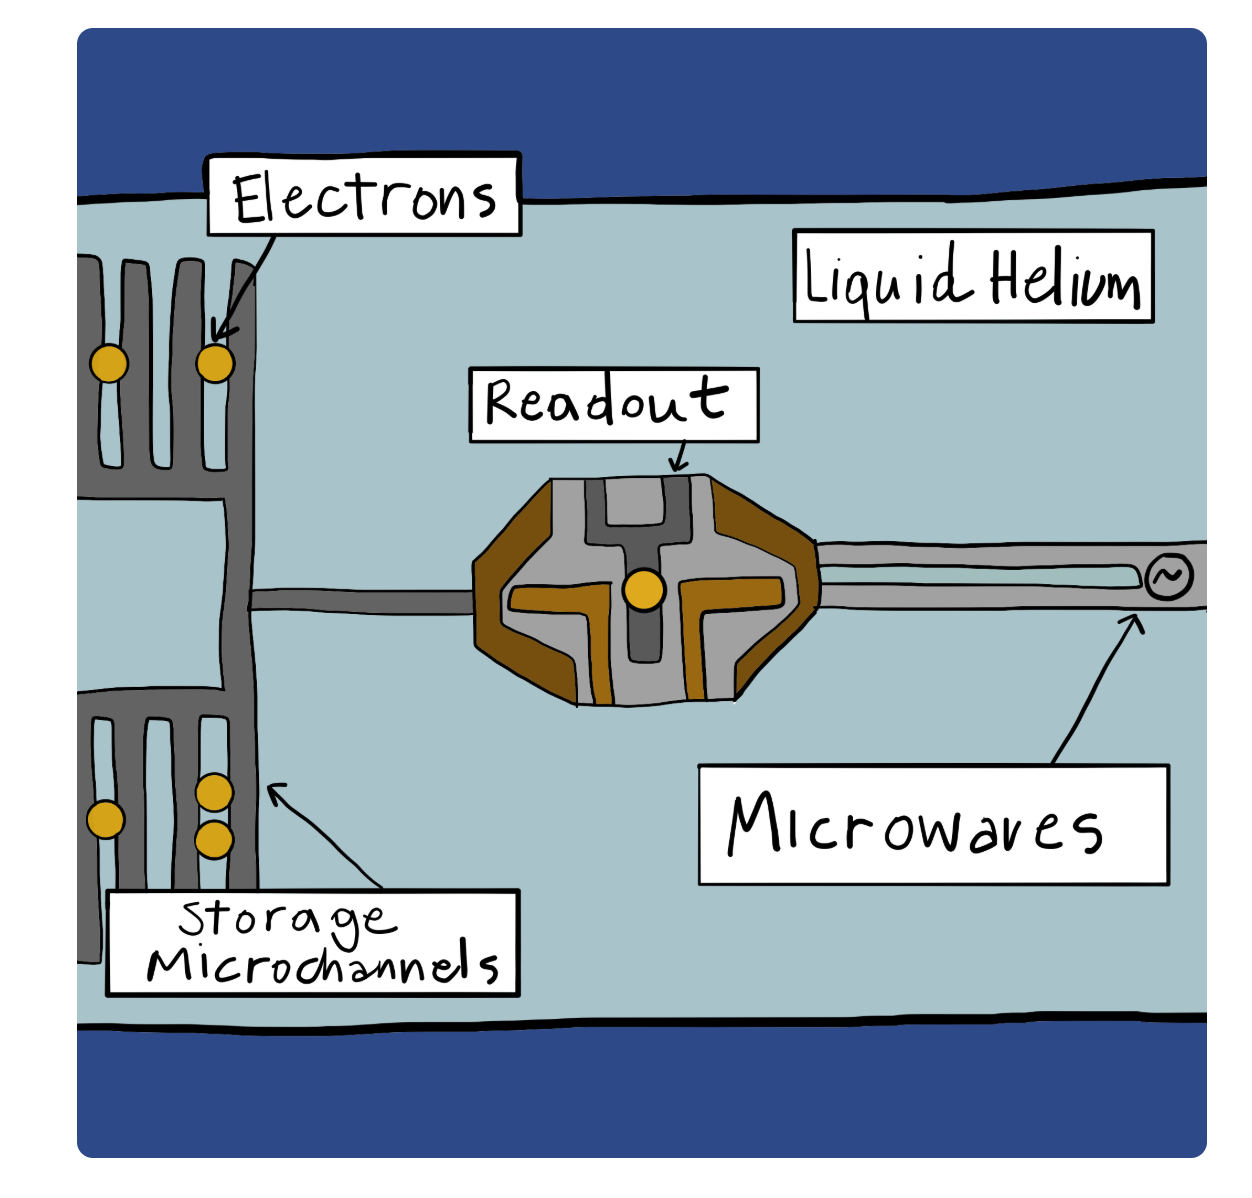
\includegraphics[width=1.2\textwidth]{qcfigures/nordicquantumfig3.png}
      \end{center}
\end{columns}
      \end{footnotesize}
    }


\frame
    {
      \frametitle{Operations for quantum computing}
	
      \begin{footnotesize}
     \begin{columns}
       \column{5.0cm}
Quantum information can be encoded in a number of ways using single electrons. Currently, we are working with the side-to-side(lateral) quantum motion of the electron in the engineered trap. This motion can either be in its lowest energy state, the ground state, or in a number of higher-energy excited states. This electron motion also provides the readout capabilities for the ultimate goal of building a large-scale quantum computer based on the electron's magnetic moment (spin).       
\column{5cm}
      \begin{center}
	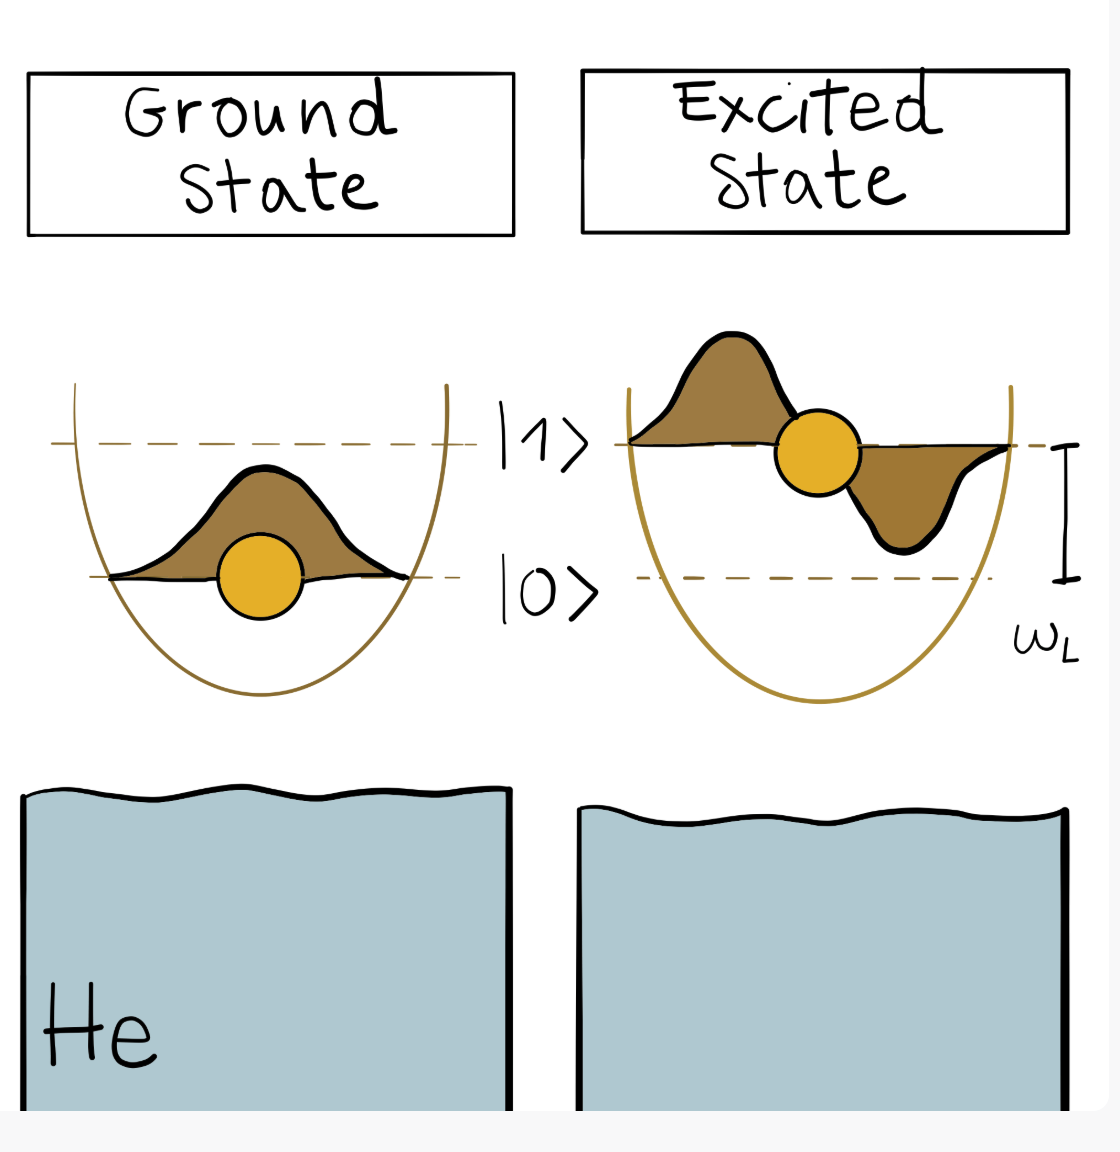
\includegraphics[width=1.2\textwidth]{qcfigures/nordicquantumfig4.png}
      \end{center}
\end{columns}
      \end{footnotesize}
    }
    
\section{Experiment and theory}



\begin{frame}[plain,fragile]
\frametitle{Experimental setup I}

\vspace{6mm}

% inline figure
\centerline{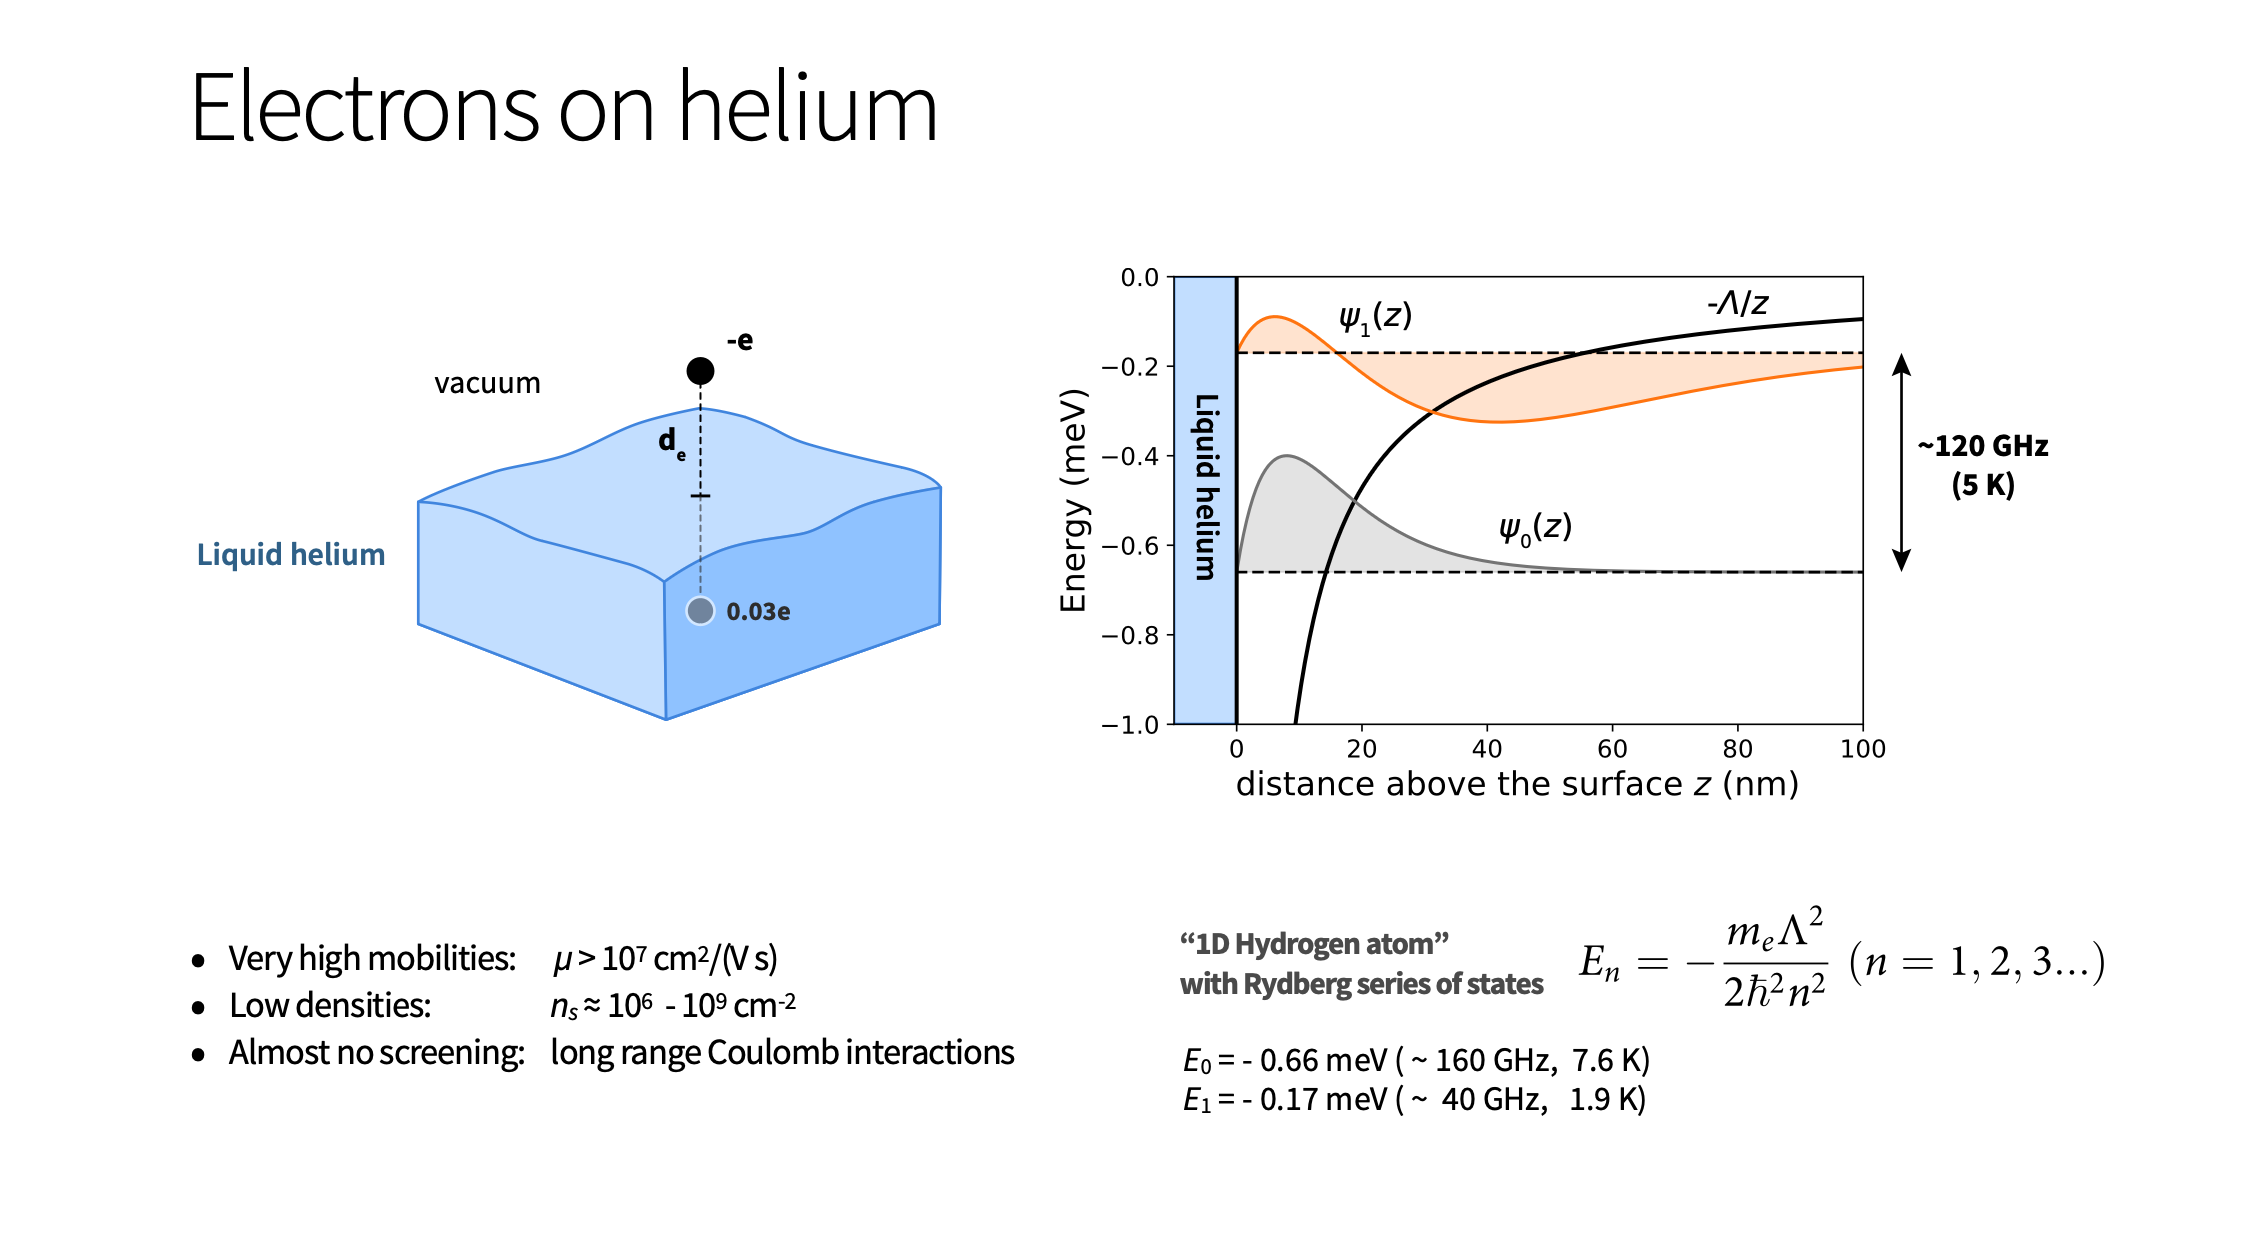
\includegraphics[width=1.3\linewidth]{qcfigures/Elhelium1.png}}

\vspace{6mm}
\end{frame}

\begin{frame}[plain,fragile]
\frametitle{More on experimental setup II}

\vspace{6mm}

% inline figure
\centerline{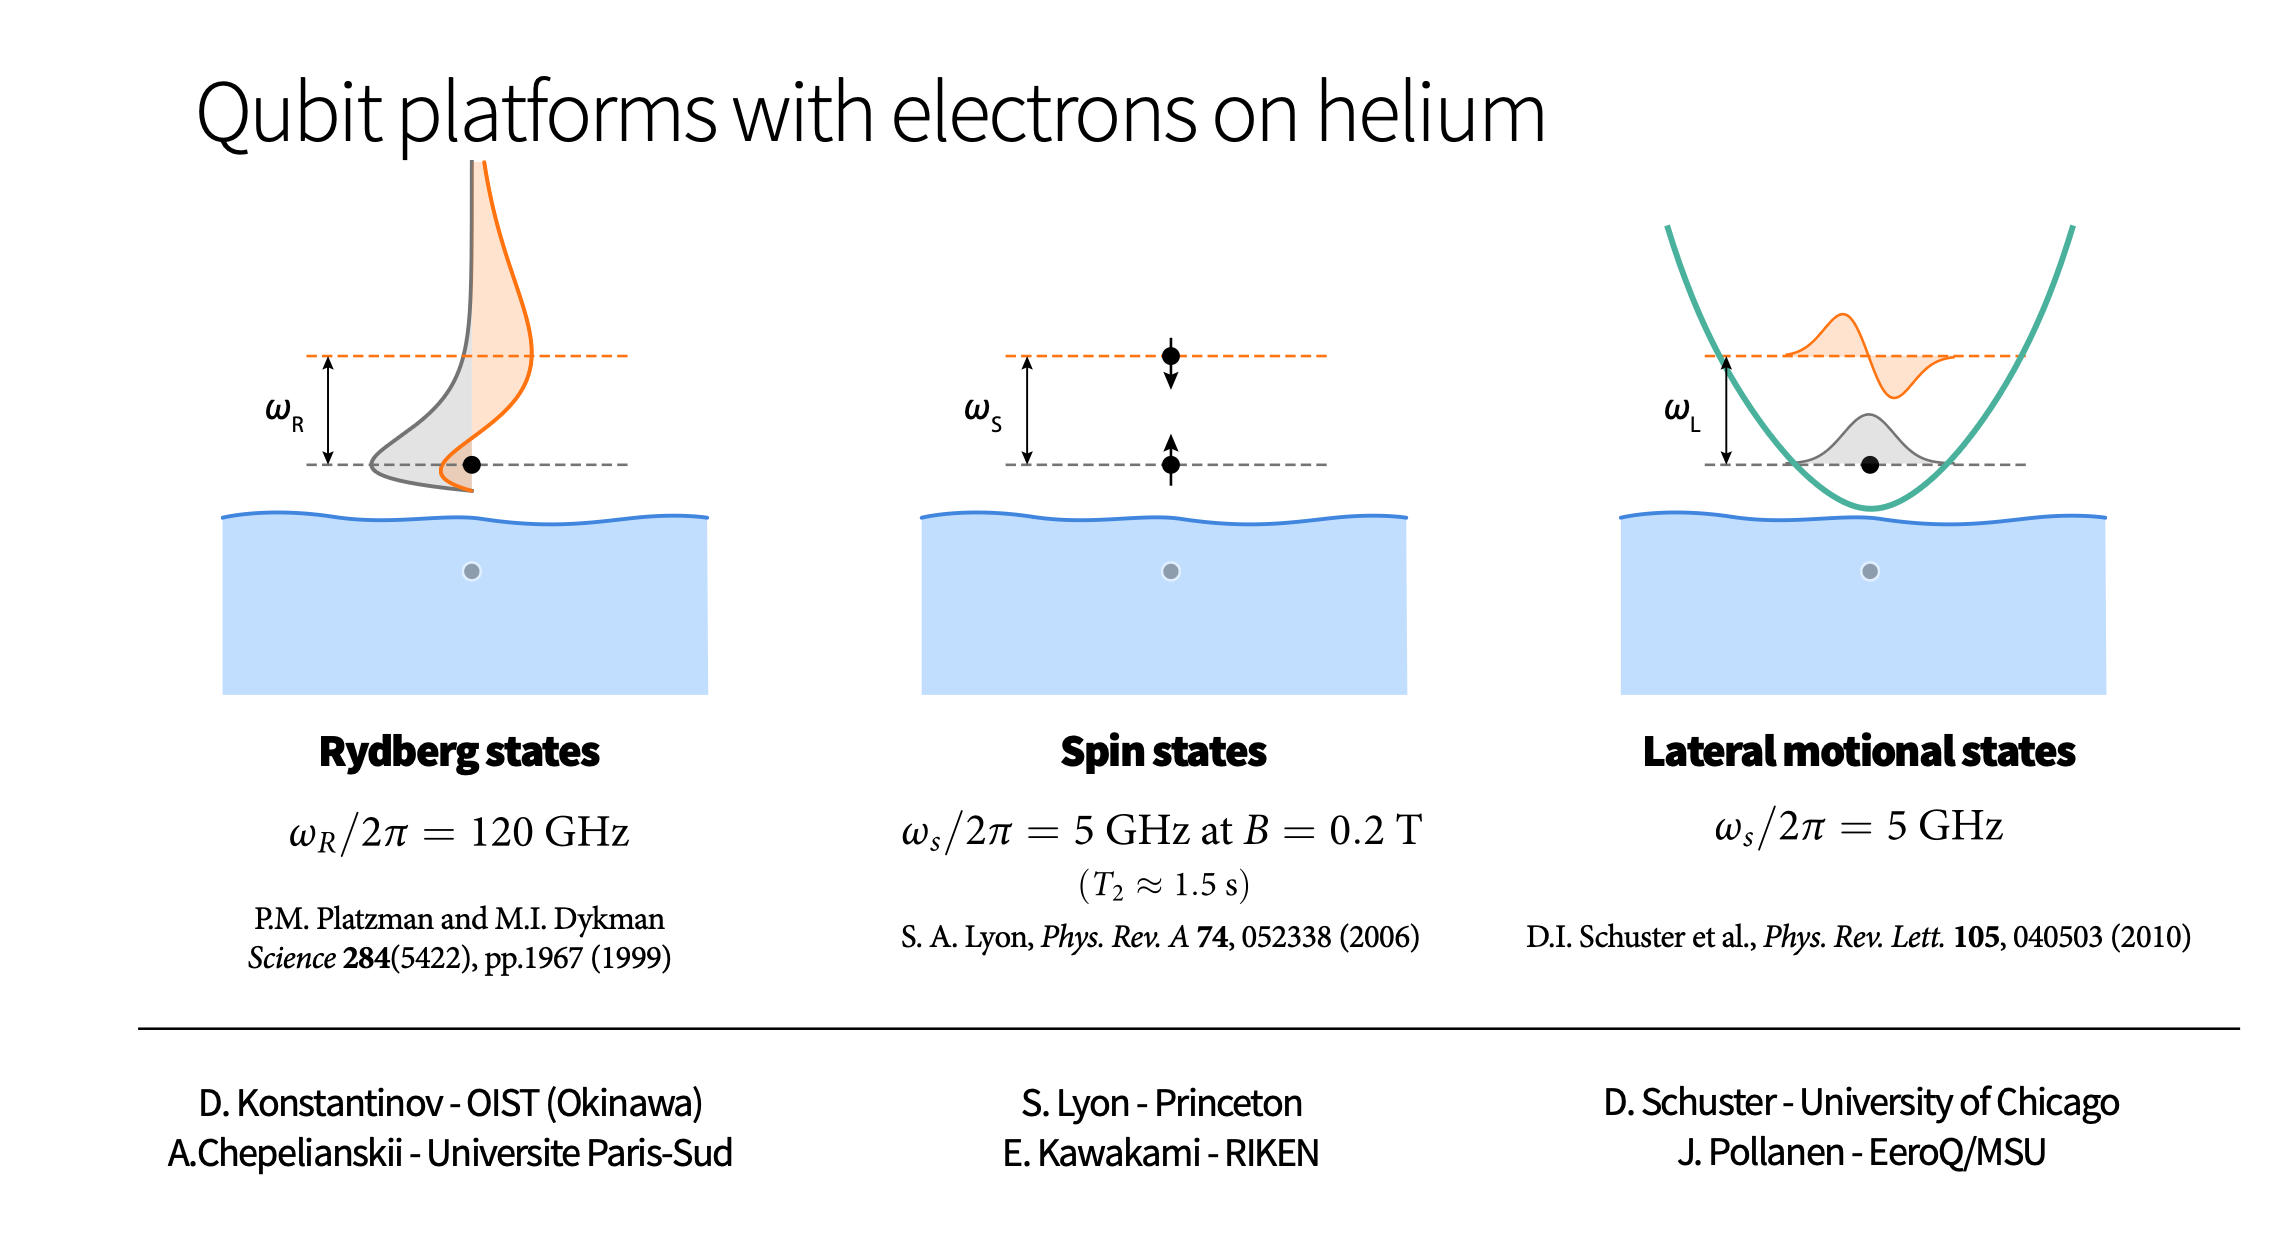
\includegraphics[width=1.3\linewidth]{qcfigures/Elhelium2.png}}

\vspace{6mm}
\end{frame}

\begin{frame}[plain,fragile]
\frametitle{More on experimental setup III}

\vspace{6mm}

% inline figure
\centerline{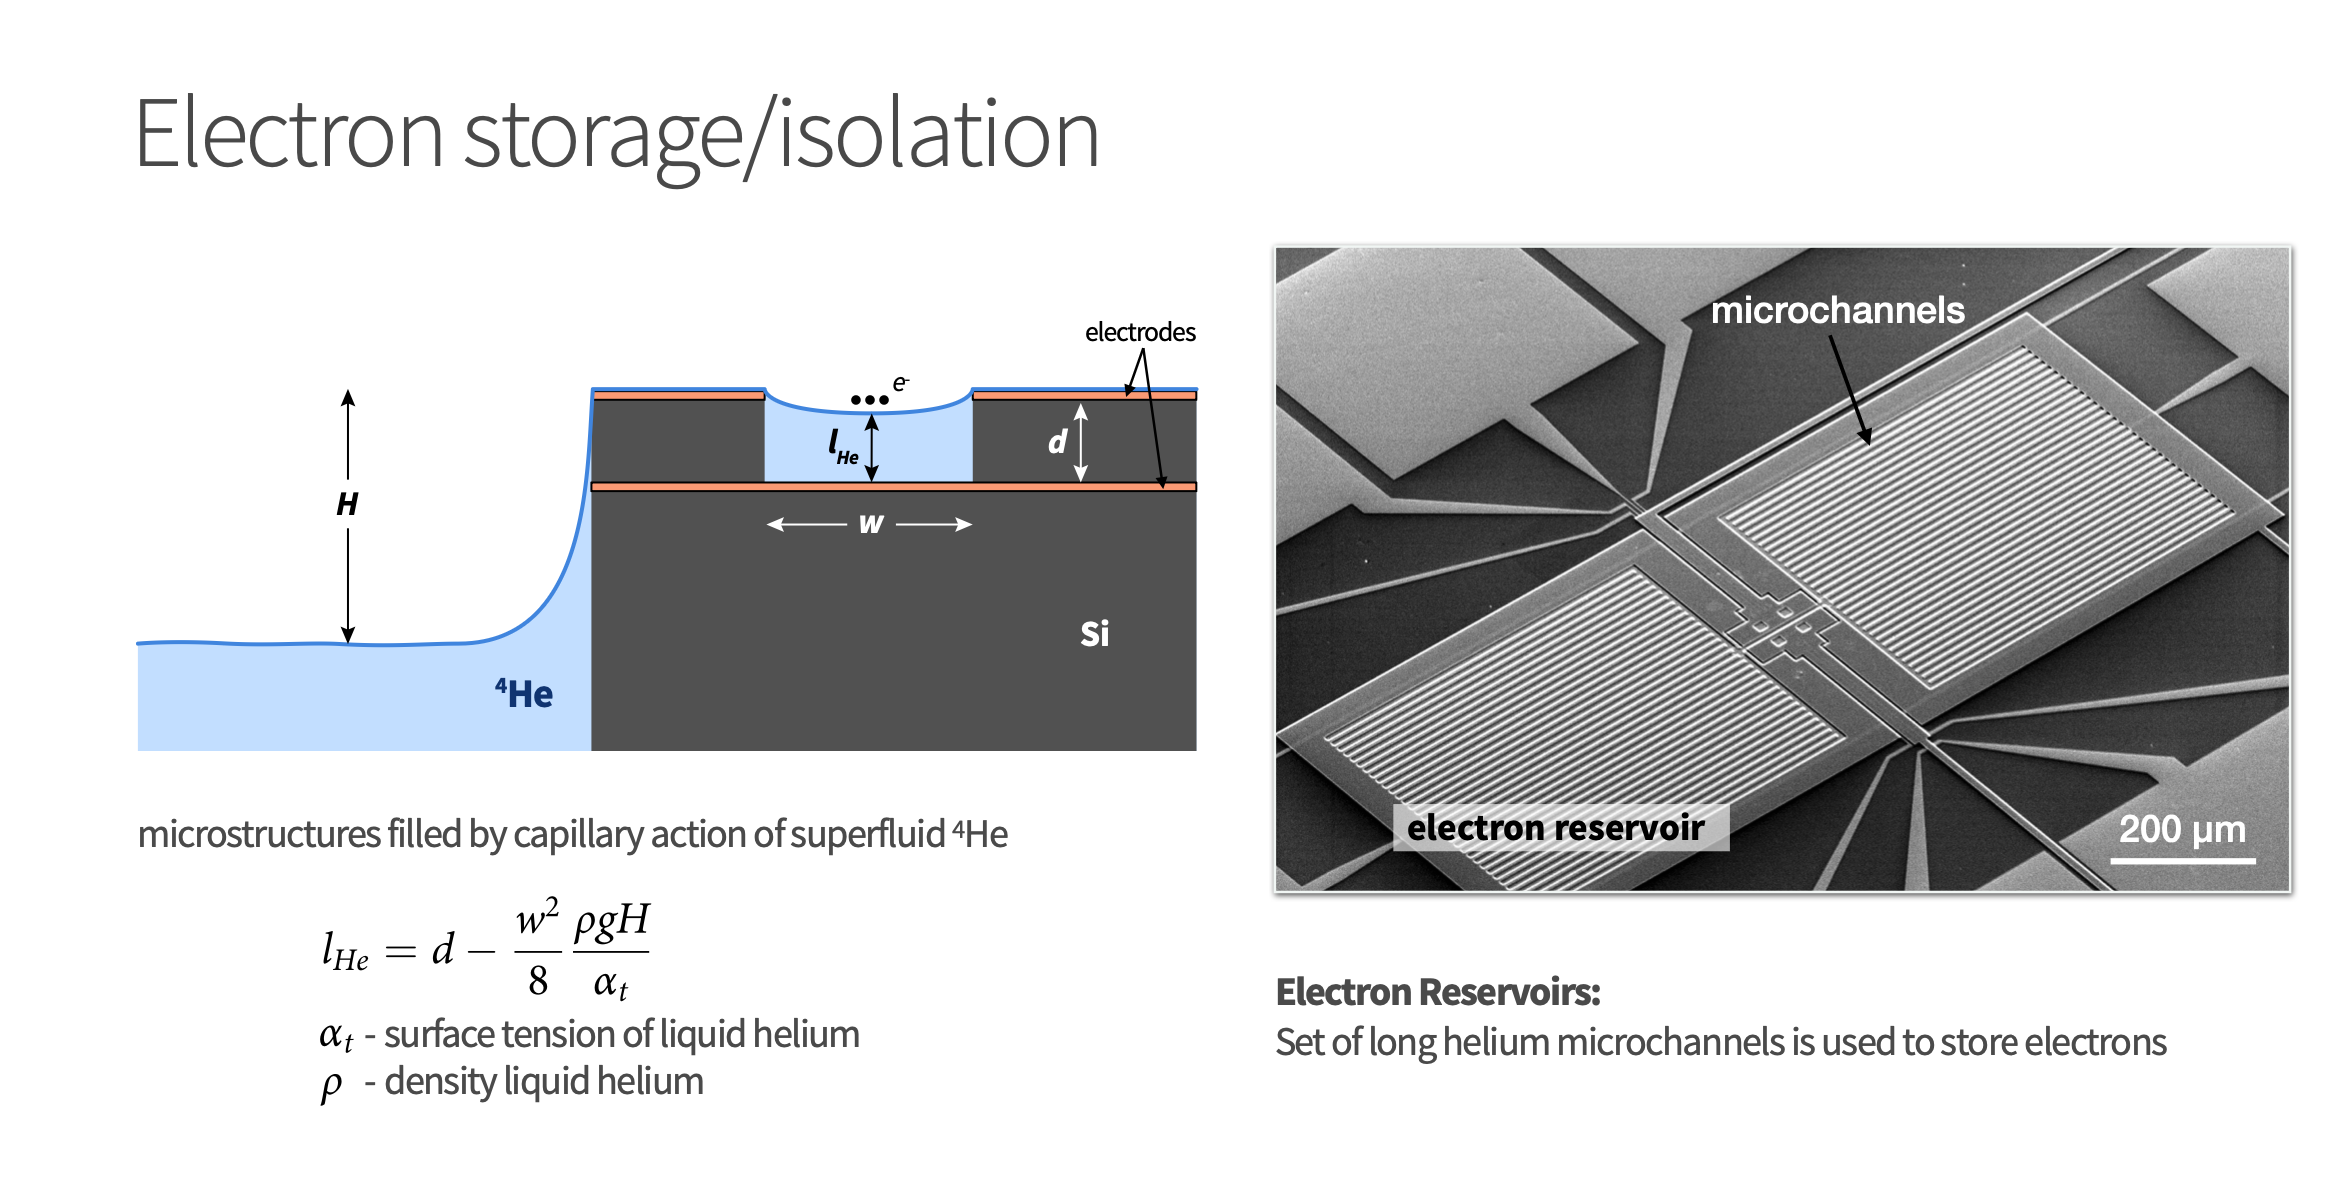
\includegraphics[width=1.3\linewidth]{qcfigures/Elhelium3.png}}

\vspace{6mm}
\end{frame}

\frame
    {
      \frametitle{Final experimental setup}
	
      \begin{footnotesize}
     \begin{columns}
       \column{5.0cm}
\begin{enumerate}
\item (a) Microdevice where two electrons are trapped in a double-well potential created by electrodes 1-7. The read-out is provided by two superconducting resonators dispersively coupled to  electron's in-plane motional states.

\item (b) Coupling constants from each individual electrode beneath the helium layer.

\item (c+d) The electron's energy in a  double-well electrostatic potential. 
\end{enumerate}

\column{6cm}
      \begin{center}
	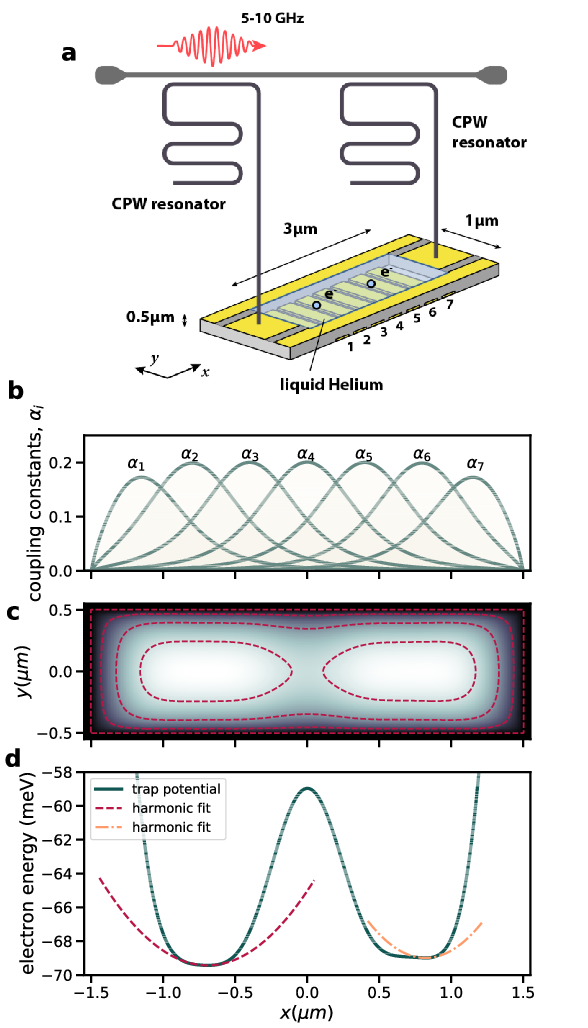
\includegraphics[width=0.65\textwidth]{qcfigures/figure1.png}
      \end{center}
\end{columns}
      \end{footnotesize}
    }



\begin{frame}[plain,fragile]
\frametitle{Quantum mechanical many-body problems (nuclear physics example here)}

\vspace{6mm}

% inline figure
\centerline{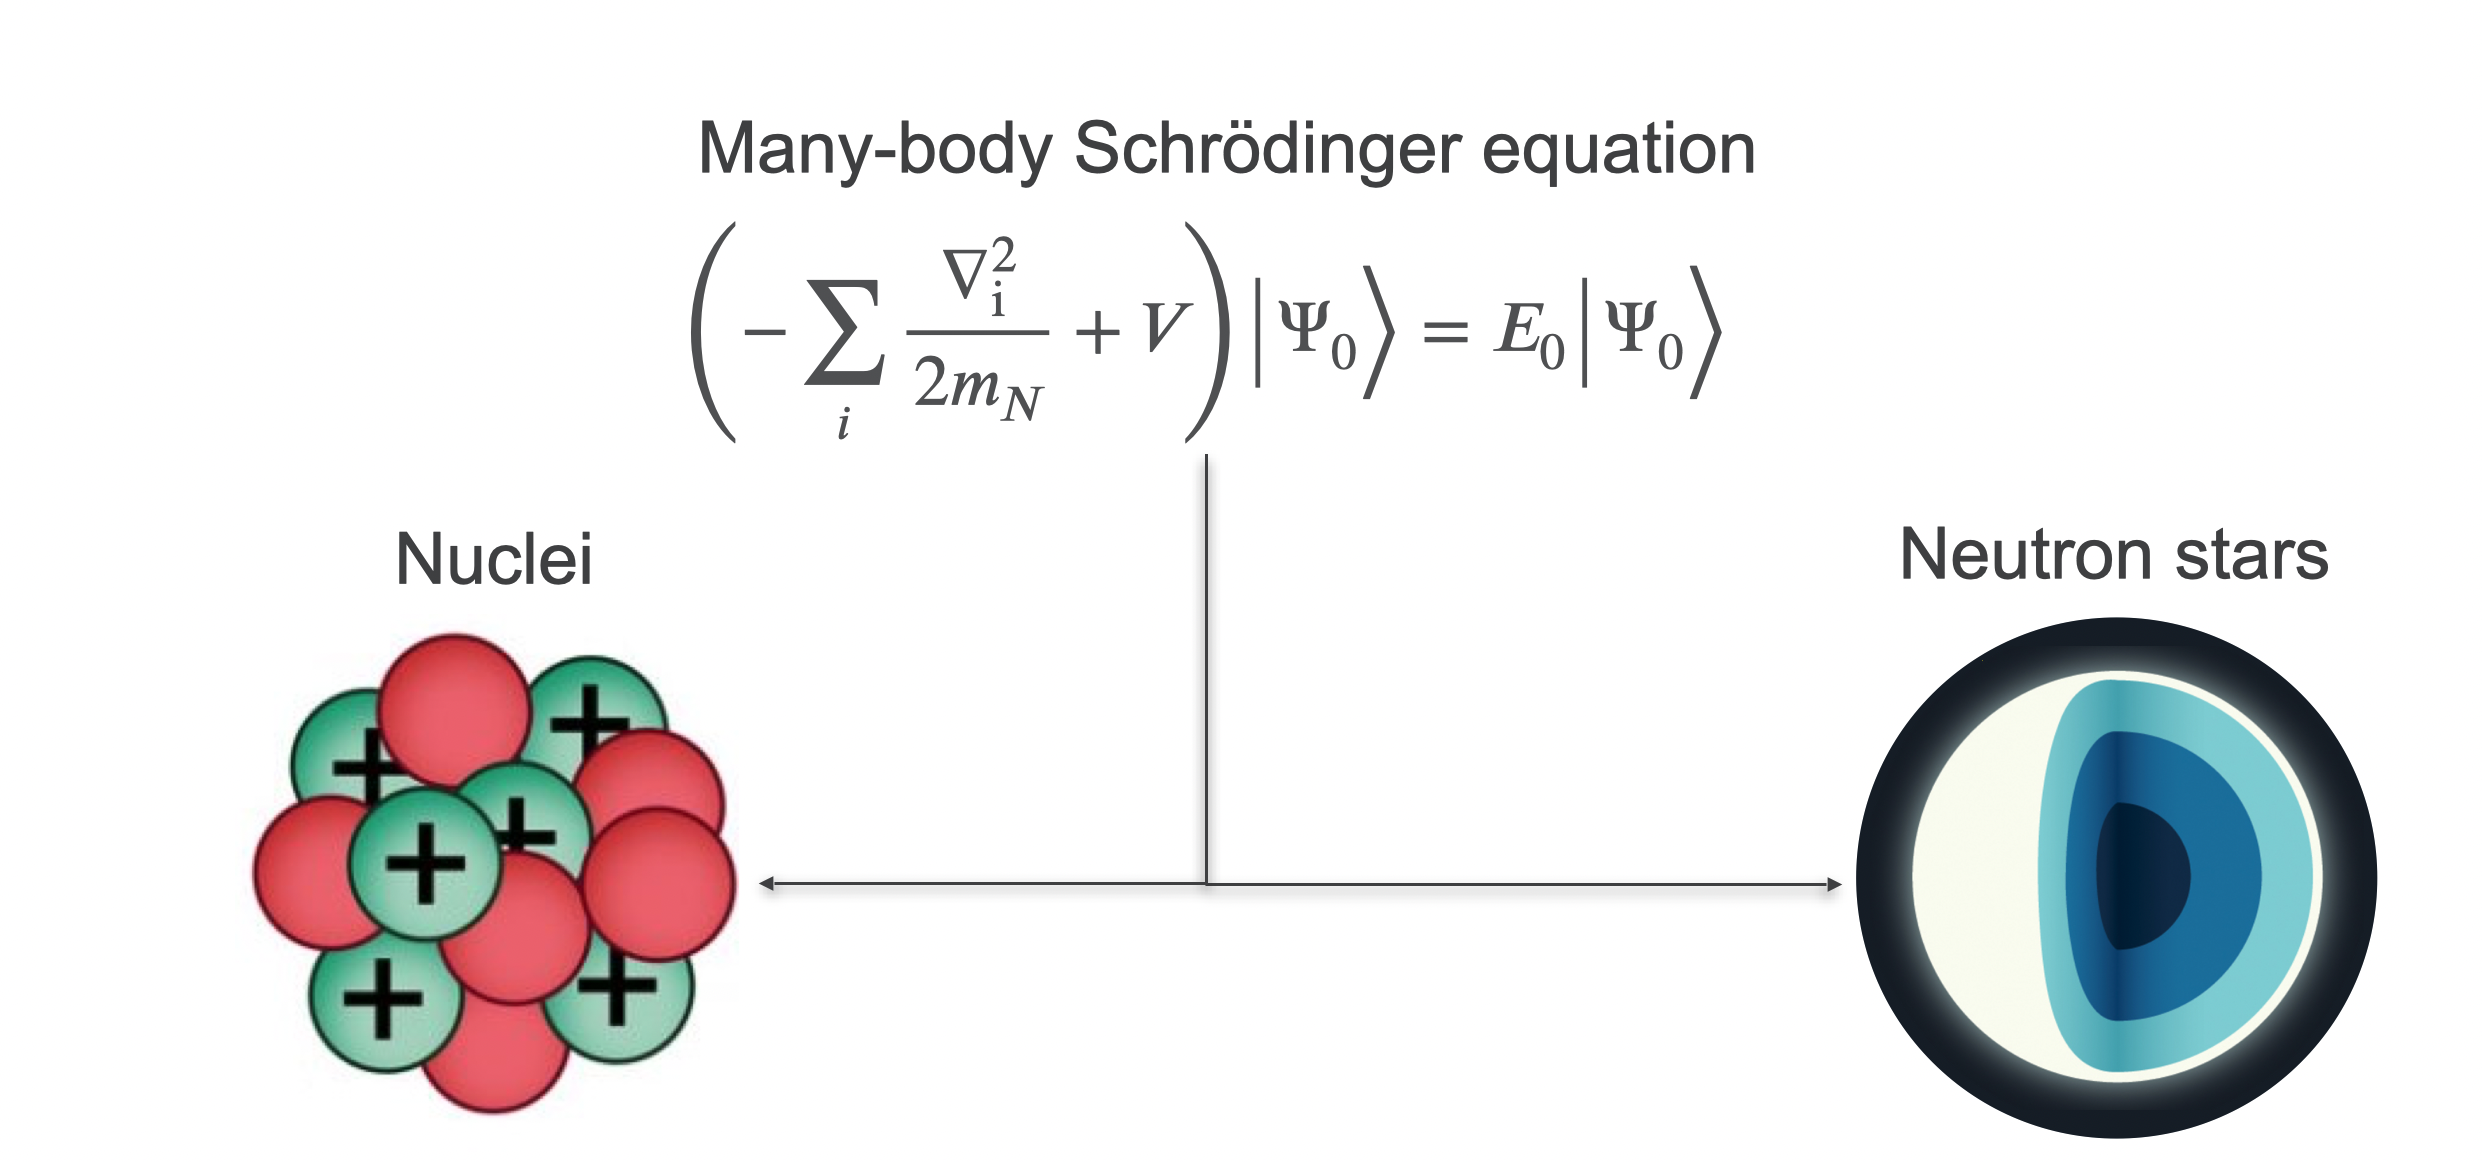
\includegraphics[width=1.1\linewidth]{qcfigures/mbpfig1.png}}

\vspace{6mm}
\end{frame}

\begin{frame}[plain,fragile]
\frametitle{Curse of dimensionality}

\vspace{6mm}

% inline figure
\centerline{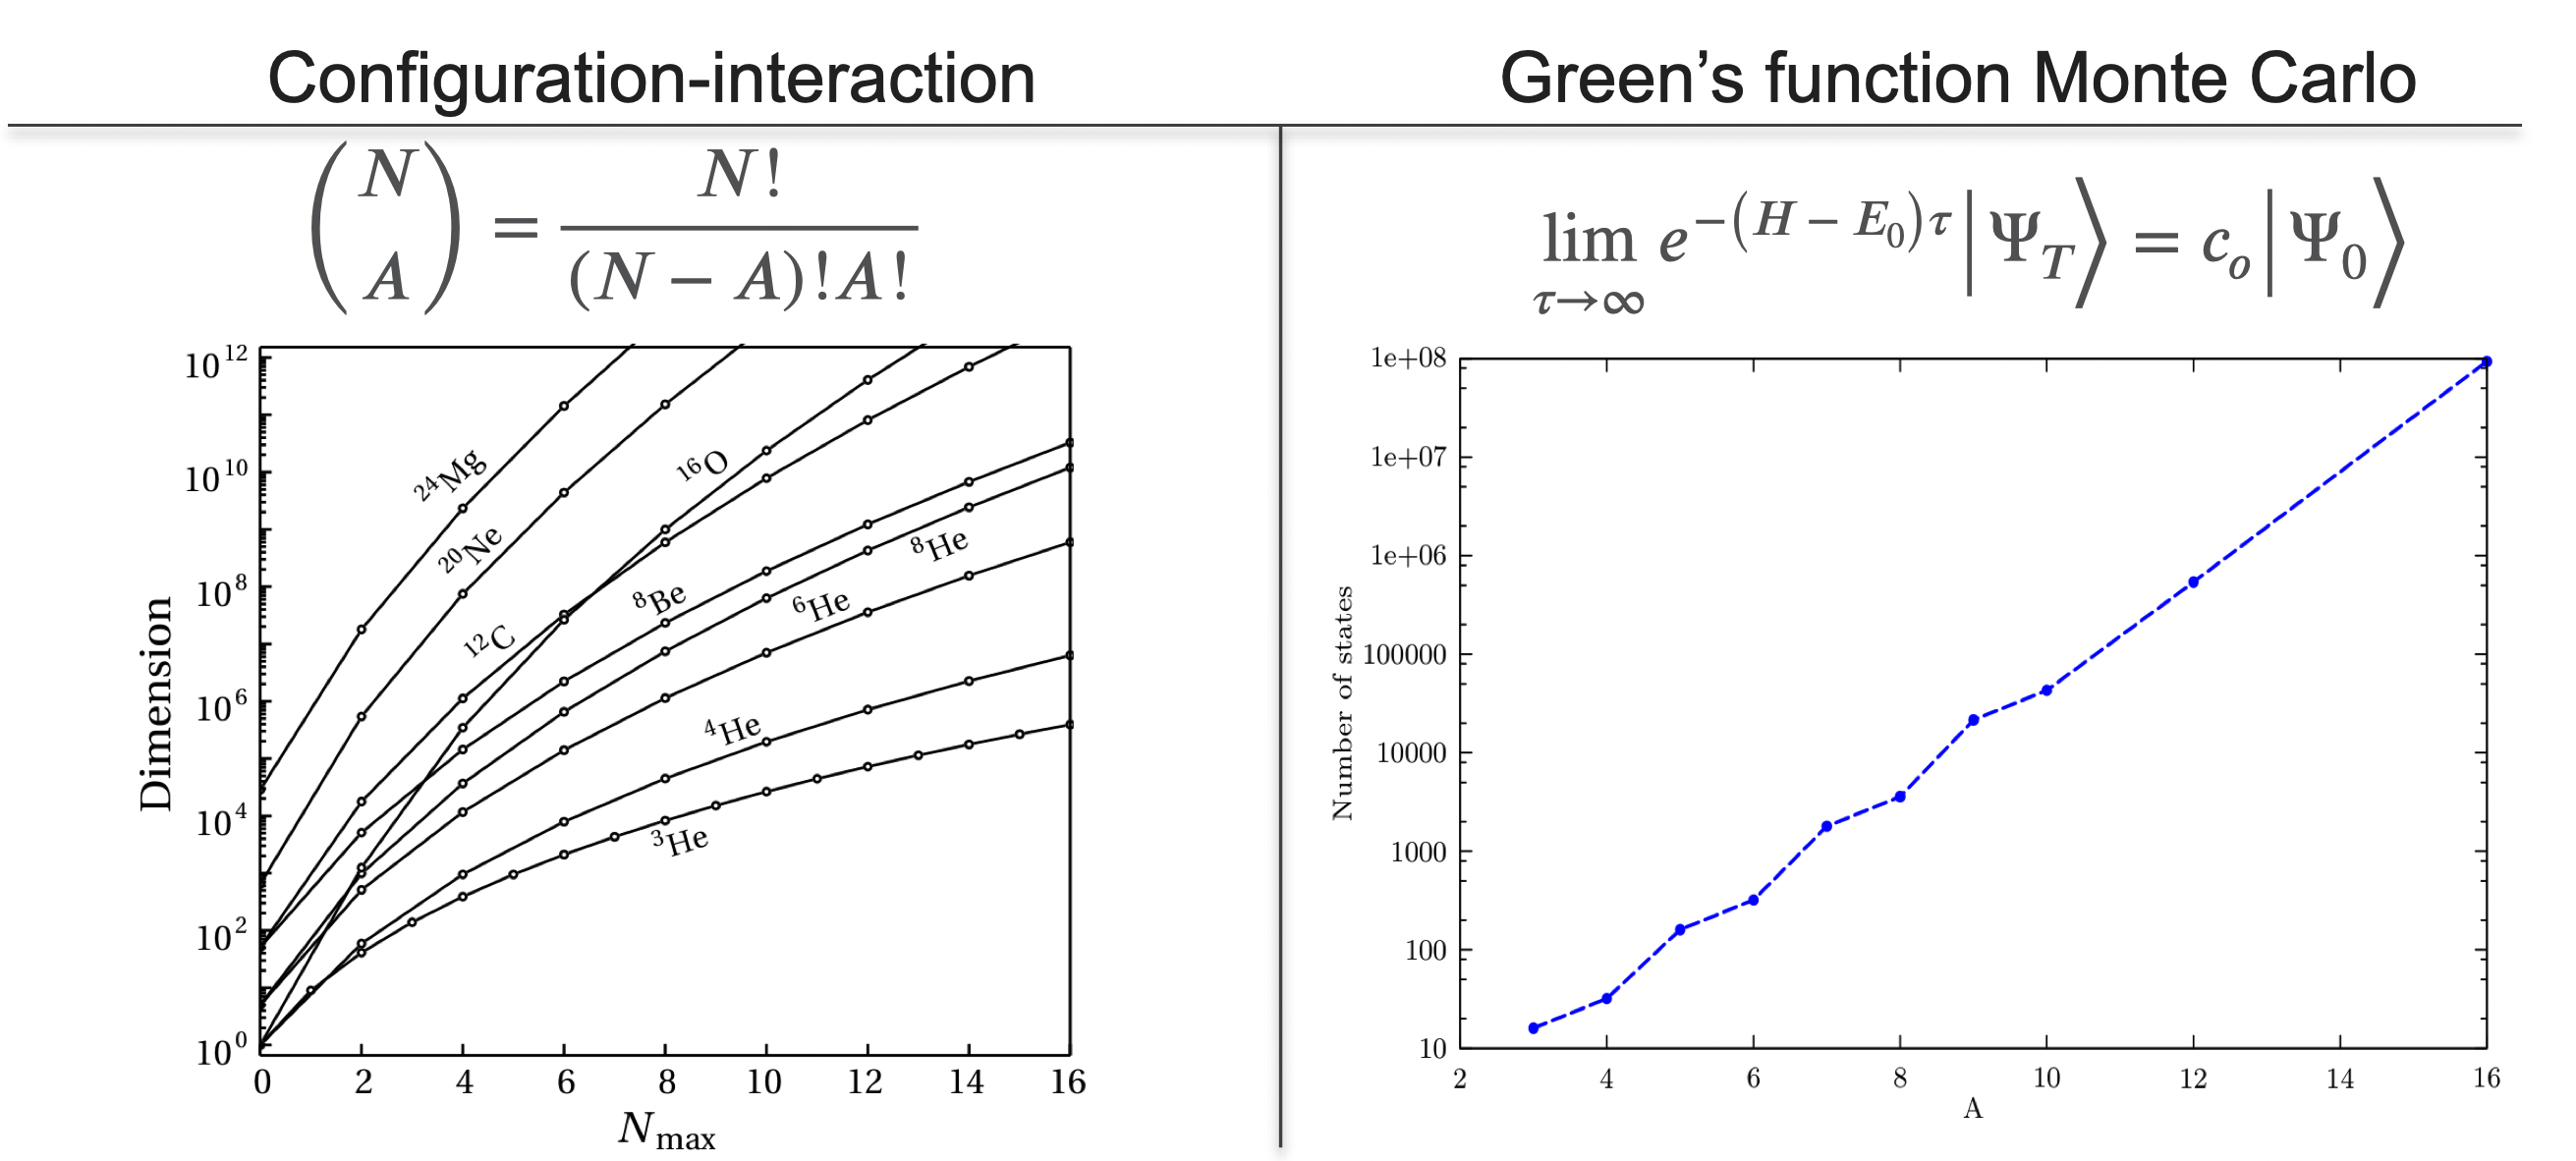
\includegraphics[width=1.0\linewidth]{qcfigures/mbpfig2.png}}

\vspace{6mm}
\end{frame}

\begin{frame}[plain,fragile]
\frametitle{\href{{https://journals.aps.org/prresearch/pdf/10.1103/PhysRevResearch.5.033062}}{Dilute neutron star matter from neural-network quantum states by Fore et al, Physical Review Research 5, 033062 (2023)} at density $\rho=0.04$ fm$^{-3}$}

\begin{block}{}

\vspace{6mm}

% inline figure
\centerline{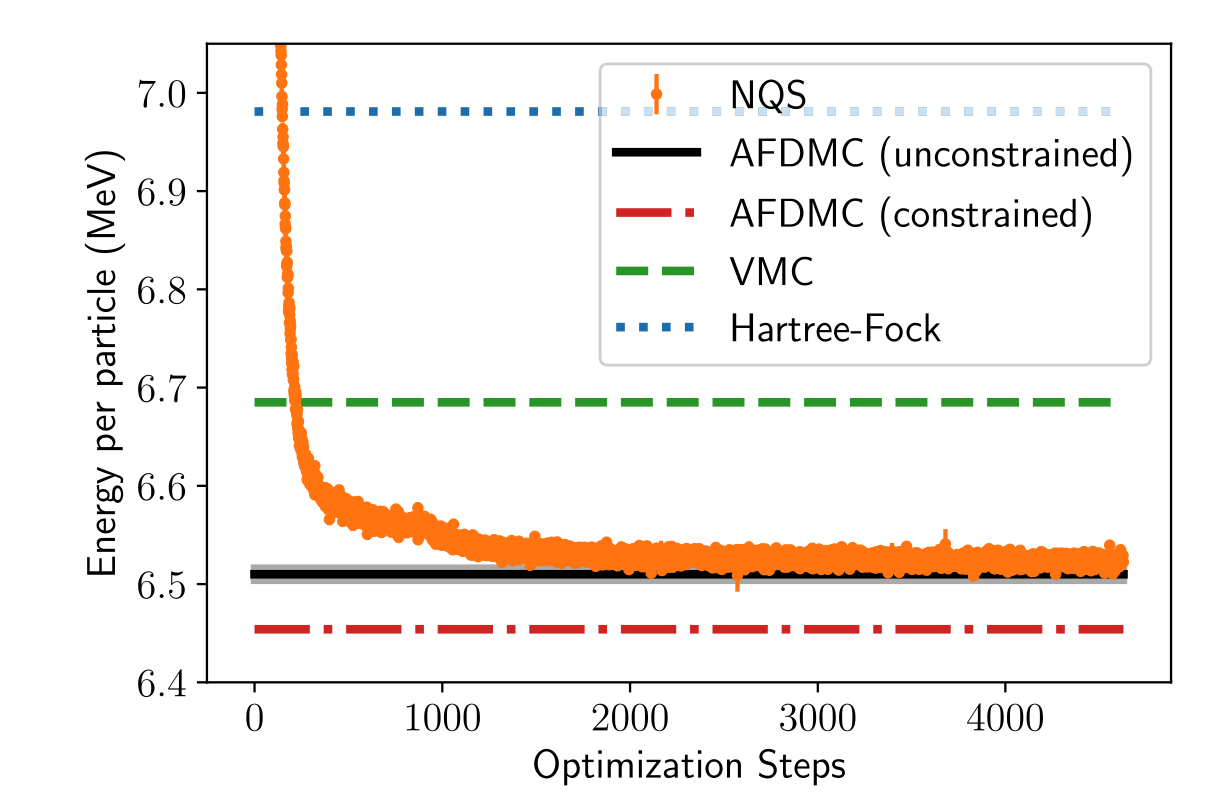
\includegraphics[width=0.9\linewidth]{qcfigures/nmatter.png}}

\vspace{6mm}

\end{block}
\end{frame}

\begin{frame}[plain,fragile]
\frametitle{Entanglement}

\begin{block}{}
\href{{https://link.springer.com/content/pdf/10.1007/s11232-007-0098-9.pdf}}{Entanglement} is the fundamental characteristic that distinguishes
quantum systems composed of two or more coupled objects from their
classical counterparts. The study of entanglement in precisely
engineered quantum systems with countably many degrees of freedom is
at the forefront of modern physics and is a key resource in quantum
information science (QIS). This is particularly true in the
development of two-qubit logic for quantum computation.
\end{block}

\begin{block}{}
The
generation of two-qubit entanglement has been demonstrated in a wide
variety of physical systems used in present-day quantum computing,
including superconducting circuits, trapped
ions, semiconductor quantum dots, color-center
defects in diamond, and neutral atoms in optical
lattices, just to name a few.
\end{block}
\end{frame}

\begin{frame}[plain,fragile]
\frametitle{More on Entanglement}

\begin{block}{}
Generating an entanglement between two quantum systems rely on
exploiting interactions in a controllable way. The details in the
interaction Hamiltonian between two systems defines the protocol
schemes for two-qubit logic.
\end{block}

\begin{block}{}
In  superconducting circuits the
interaction between qubits may arise from direct capacitive coupling
between circuit elements or by indirect coupling of two qubits to a
common resonator (virtually populating resonator mode) which results
in a non-local Hamiltonian in the form of exchange
interaction. This allow to implement various
schemes for entanglement, such as controlled-phase
gate, resonator-induced phase
gate, cross-resonance gates etc.
\end{block}
\end{frame}



\begin{frame}[plain,fragile]
\frametitle{Quantum dots and the Coulomb interaction}

\begin{block}{}
Coulomb interaction governed entanglement can be realized in
the system of electrons on the surface of superfluid helium, where
qubit states are formed by in-plane lateral motional or out-of plane
Rydberg states. Trapped near the surface of liquid helium these states
have different spatial charge configurations and the wavefunctions of
different electrons do not overlap.
\end{block}

\begin{block}{}
This results in a strong exchange
free Coulomb interaction which depends on the states of the
electrons. The lack of disorder in the systems
also leads to slow electron decoherence, which has attracted interest
to the system as a candidate for quantum information
processing.
\end{block}
\end{frame}

\begin{frame}[plain,fragile]
\frametitle{Electrons on helium as another qubit platform}


\begin{block}{Two qubit gates}
The static Coulomb interaction arises from a virtual photon exchange
 process between two charge particles according to quantum
 electrodynamics. This results in a correlated motion of two charges generating quantum entanglement. 
\end{block}
\end{frame}

\begin{frame}[plain,fragile]
\frametitle{Surface state electrons (SSE)}

\begin{block}{}
Surface state electrons (SSE) 'floating' above liquid helium
originates from quantization of electron's perpendicular to the
surface motion in a trapping potential formed by attractive force from
image charge and a large $\sim$ 1 eV barrier at the liquid-vacuum
interface. At low temperatures the SSE are trapped in the lowest
Rydberg state for vertical motion some 11 nm above the helium surface,
which is perfectly clean and has a permittivity close to that of
vacuum.
\end{block}

\begin{block}{}
The weak interaction with the enviroment, which is mainly governed
by interaction with quantized surface capillary waves (ripplons) and
bulk phonons, ensures long coherence times - a vital ingredient for
any qubit platform. 
\end{block}
\end{frame}

\begin{frame}[plain,fragile]
\frametitle{Calculational details}

\begin{align}
\hat{H} &=\frac{\hat{p}_1^2}{2} + \sum_{i = 1}^7 V_i\alpha_i[\hat{x}_1] + \frac{\hat{p}_2^2}{2} + \sum_{i = 1}^7 V_i\alpha_i[\hat{x}_2] + \frac{\kappa}{\sqrt{(\hat{x}_1-\hat{x}_2)^2 + a^2}}\\
&= h[\hat{p}_1,\hat{x}_1] + h[\hat{p}_2,\hat{x}_2] + u[\hat{x}_1,\hat{x}_2]
\end{align}

\vspace{6mm}

% inline figure
\centerline{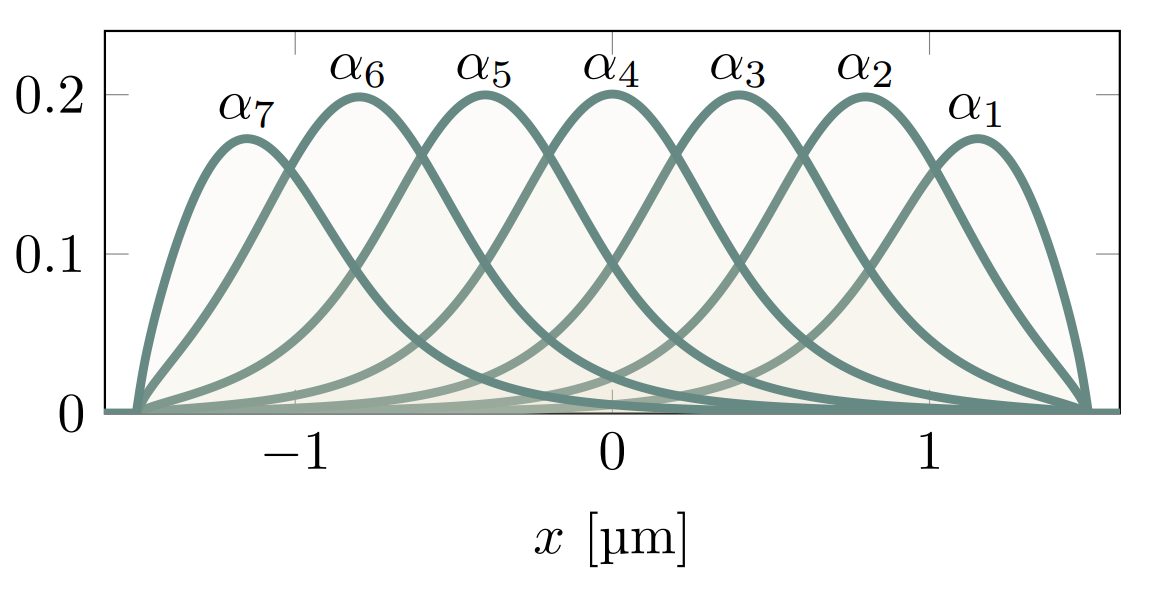
\includegraphics[width=0.8\linewidth]{qcfigures/well_basis.png}}

\vspace{6mm}
\end{frame}

\begin{frame}[plain,fragile]
\frametitle{Calculational details}

\begin{align}
\hat{H} &= \frac{\hat{p}_1^2}{2} + v[\hat{x}_1] + \frac{\hat{p}_2^2}{2} + v[\hat{x}_2] + \frac{\kappa}{\sqrt{(\hat{x}_1-\hat{x}_2)^2 + a^2}}\\
&= h[\hat{p}_1,\hat{x}_1] + h[\hat{p}_2,\hat{x}_2] + u[\hat{x}_1,\hat{x}_2]
\end{align}

\vspace{6mm}

% inline figure
\centerline{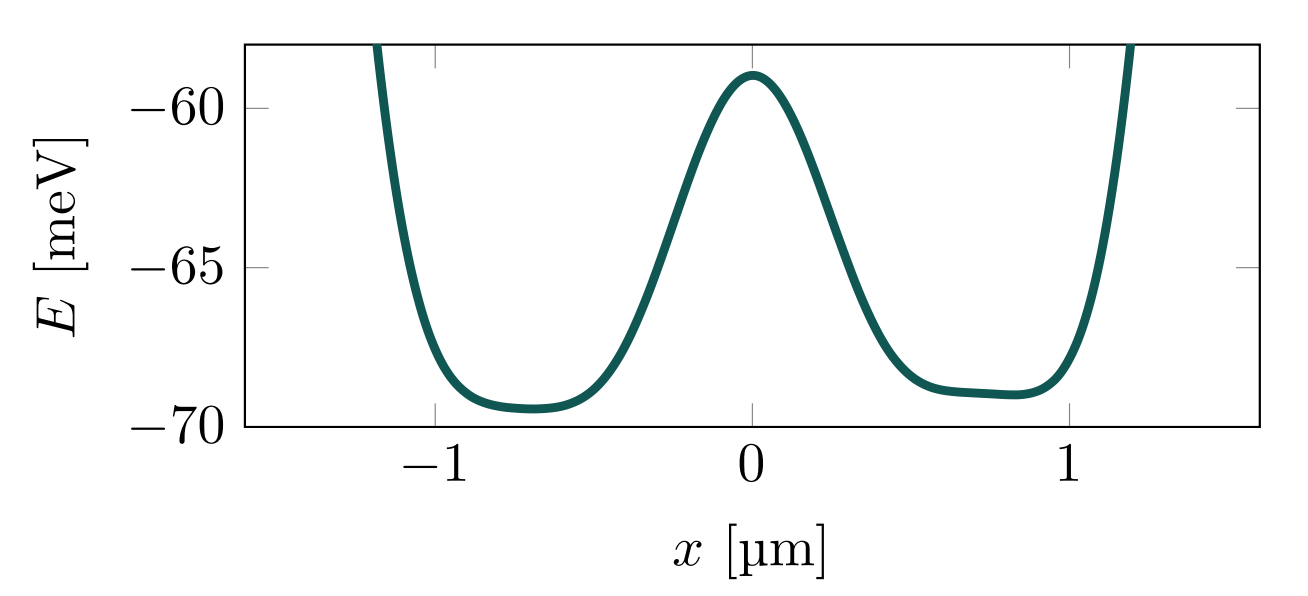
\includegraphics[width=0.8\linewidth]{qcfigures/wells.png}}

\vspace{6mm}
\end{frame}

\section{Results}



\begin{frame}[plain,fragile]
\frametitle{Results and discussions}

By adjusting the potential we can change the anharmonicities and detuning of the wells.
\begin{enumerate}
\item What values of these give interesting interactions?

\item Inspiration from superconducting qubits, see High-Contrast $ZZ$ Interaction Using Superconducting Qubits with Opposite-Sign Anharmonicity, \href{{https://journals.aps.org/prl/abstract/10.1103/PhysRevLett.125.200503}}{Zhao et al Phys. Rev. Lett. 125, 200503}
\end{enumerate}

\noindent
\end{frame}

\begin{frame}[plain,fragile]
% No title on this slide

We search for well configurations corresponding to three different types of interaction between the two electrons.

\begin{enumerate}
\item In configuration I we address both qubits independently and can thereby perform single-qubit state rotations and measurements.

\item Configurations II and III correspond to avoided level crossings between two ($E_{01}, E_{10}$) and three ($E_{11}, E_{20}, E_{02}$) energy levels respectively, where the electrons' motion becomes correlated, that is they are entangled. 
\end{enumerate}

\noindent
Both anharmonicity and detuning changes with the shape of our well.
We create a voltage parameterization
\begin{equation}
V(\lambda) = (1-\lambda)V_\mathrm{I} + \lambda V_\mathrm{III}
\end{equation}
\end{frame}

\begin{frame}[plain,fragile]
\frametitle{Configurations}
% inline figure
\centerline{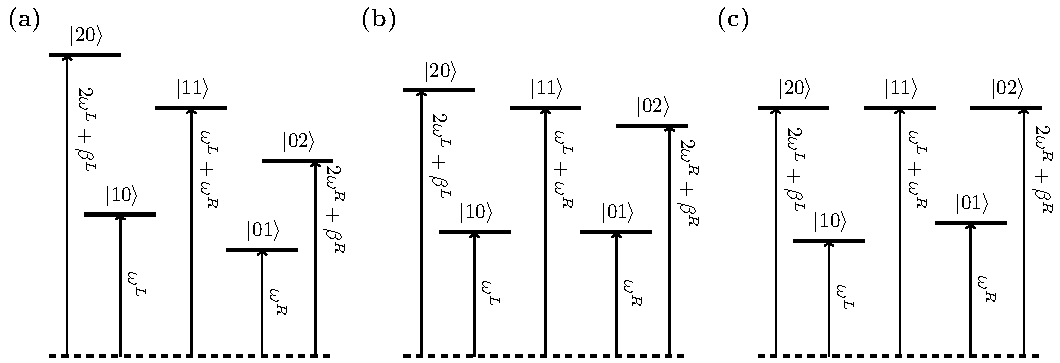
\includegraphics[width=0.8\linewidth]{qcfigures/states.pdf}}
(a) Transition frequencies in the non-interacting picture for configuration I. This configuration corresponds to a detuned
system in which all transition energies are distinguishable. (b) Transition
frequencies in configuration II. The two states $\vert 10\rangle$ and $\vert 01\rangle$ are degenerate in the
absence of interactions. (c)
Configuration III is realized when the three states $\vert 20\rangle$, $\vert 11\rangle$ and $\vert 02\rangle$ share the same transition frequency from the ground
state. 
\end{frame}


\frame
    {
      \frametitle{Probabilities}
	
      \begin{footnotesize}
     \begin{columns}
       \column{5.0cm}
Probability distributions of the first four 
states in the left and right wells for all three configurations.

The position of the distributions are shifted along the $y$-axis
to reflect their individual energies. The effective potentials for each subsystem, i.e., the well potential set up by
the electrodes plus the mean-field contribution from the other
electron, are plotted as dashed lines.
\column{6cm}
      \begin{center}
	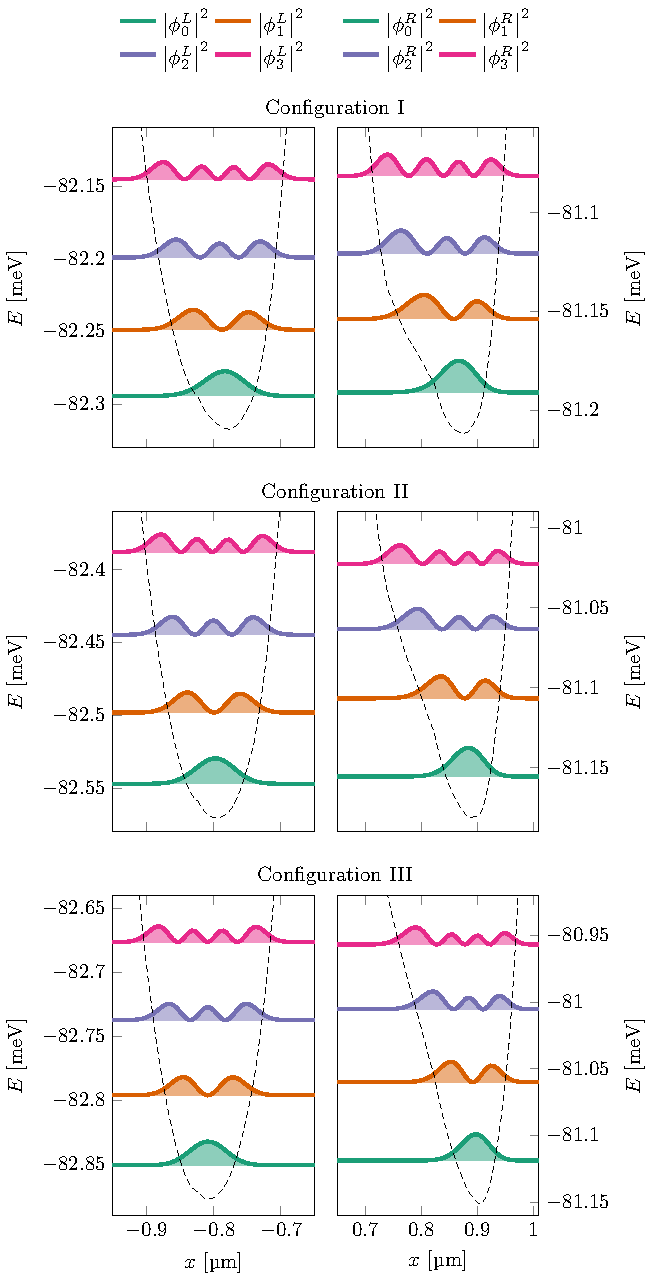
\includegraphics[width=0.6\textwidth]{qcfigures/probability.pdf}
      \end{center}
\end{columns}
      \end{footnotesize}
    }


\frame
    {
      \frametitle{Coefficients of states}
	
      \begin{footnotesize}
     \begin{columns}
       \column{5.0cm}
\begin{itemize}
\item[(a)] Two-body wave function coefficients of the six lowest energy eigenstates for config I

\item[(b)] Coefficients for configuration II. The first and second excited eigenstates are close to maximally entangled.

\item[(c)] Coefficients for configuration III. Here, the third, fourth and fifth excited eigenstates are entangled.

\end{itemize}

\column{6cm}
      \begin{center}
	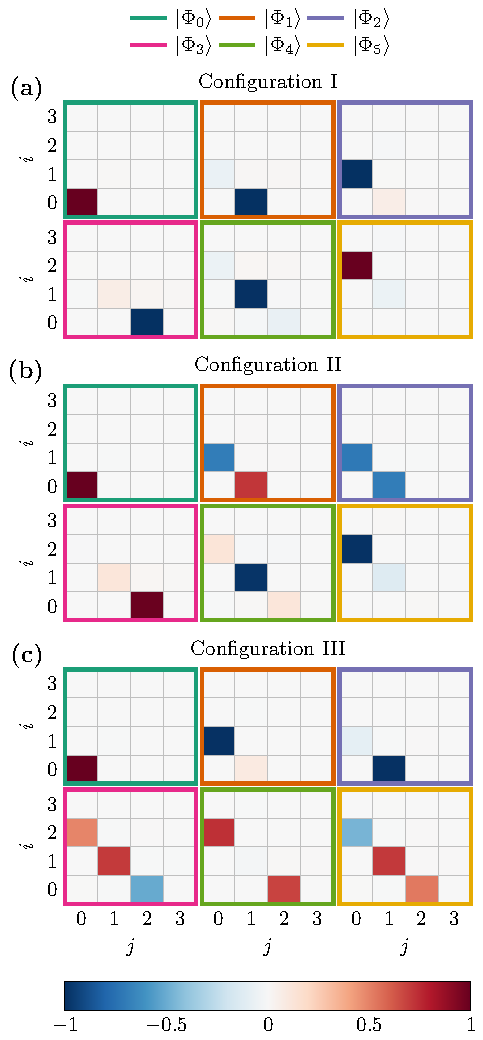
\includegraphics[width=0.6\textwidth]{qcfigures/coeffs.pdf}
      \end{center}
\end{columns}
      \end{footnotesize}
    }

\frame
    {
      \frametitle{Entanglement}
	
      \begin{footnotesize}
     \begin{columns}
       \column{5.0cm}
\begin{itemize}
\item[(a)] Transition frequencies from the ground state of the five lowest excited energy eigenstates

\item[(b)] Von Neumann entropies of the same five eigenstates as functions of $\lambda$

\item[(c)] Anharmonicites of the left and right wells 
\end{itemize}

\column{6cm}
      \begin{center}
	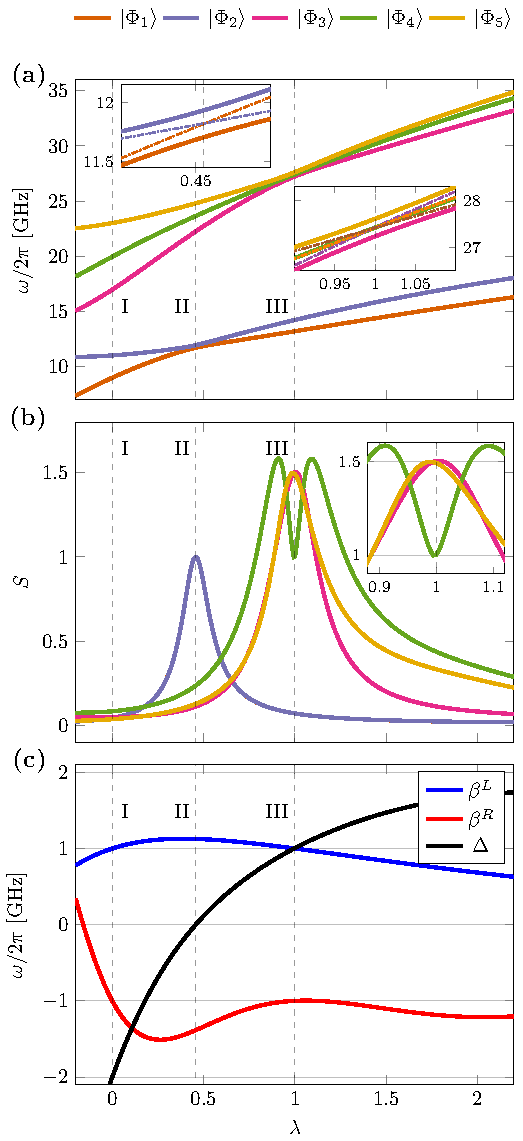
\includegraphics[width=0.6\textwidth]{qcfigures/entanglement.pdf}
      \end{center}
\end{columns}
      \end{footnotesize}
    }



\begin{frame}[plain,fragile]
\frametitle{Sensing and control of single trapped electrons}
% inline figure
\centerline{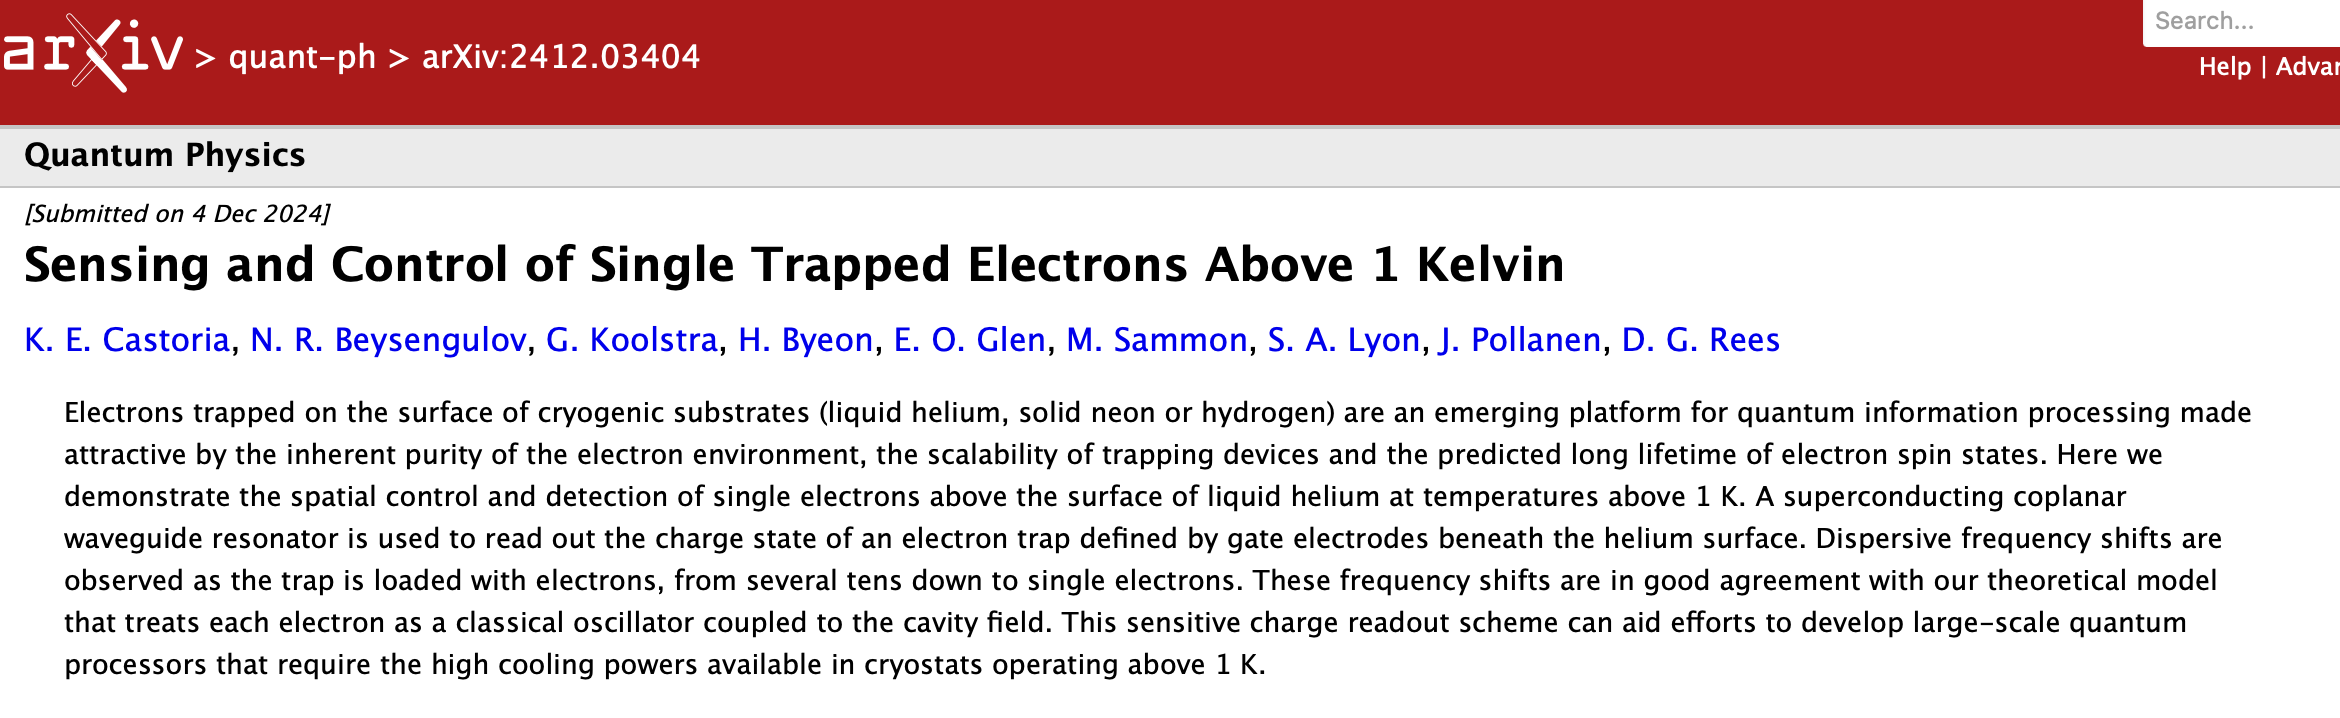
\includegraphics[width=1.2\linewidth]{qcfigures/sensing.png}}
\end{frame}


\begin{frame}[plain,fragile]
\frametitle{Entropy for two-electrons from one well to two wells}
% inline figure
%\centerline{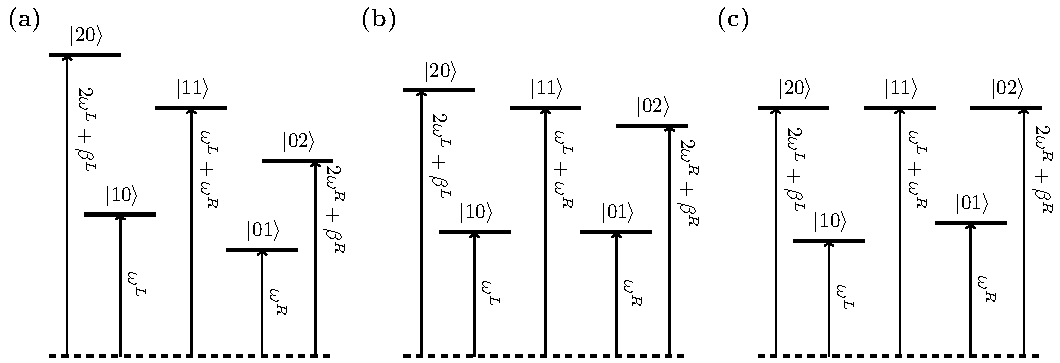
\includegraphics[width=0.8\linewidth]{qcfigures/states.pdf}}
\end{frame}


\begin{frame}[plain,fragile]
\frametitle{Expectation values of energies}
% inline figure
%\centerline{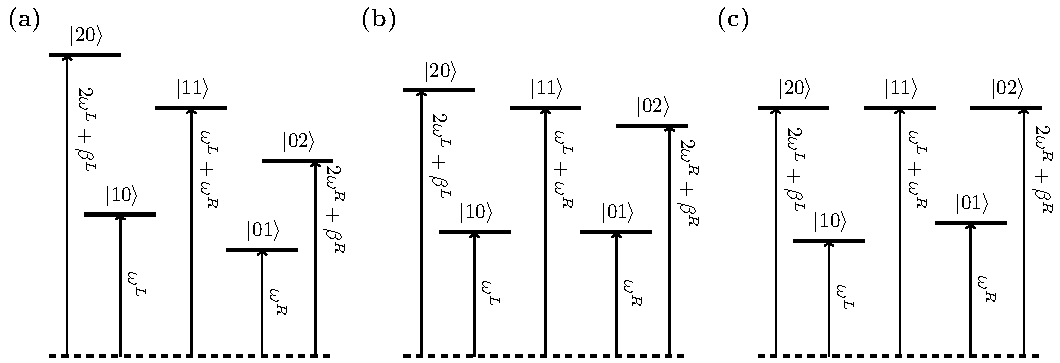
\includegraphics[width=0.8\linewidth]{qcfigures/states.pdf}}
\end{frame}




\section{Conclusions and perspectives}

\begin{frame}[plain,fragile]
\frametitle{Where we are now and future plans}

\begin{enumerate}
\item Adding time-dependent studies of two electrons in two wells

\item Studies of the time-evolution of entangled states

\item Use theory to find optimal experimental setup

\item Expect two-electron system realized experimentally in approx $1$ year, great potential for studies of quantum simulations

\item Theory for single-qubit gates and two-qubit gates  
\end{enumerate}

\noindent
\end{frame}

\begin{frame}[plain,fragile]
\frametitle{More results and Plans}

\begin{enumerate}
\item Included  two and three-dimensions (DFT basis) in order to simulate in  a more realistic way such many-body systems.

\item New time-dependent FCI code, useful up to approximately 10 particles with \textbf{effective} (and effective Hilbert space) Hamiltonians in two and three dimensions

\item Develop codes for studies of entanglement as function of time


\item Study the feasibility of various setups for quantum simulations of specific Hamiltonians

\item For larger many-body systems, study for example time-dependent CC theory
\end{enumerate}

\noindent
\end{frame}




\end{document}

